\documentclass[11pt,a4paper]{report}

% ===================== PAQUETES =====================
\usepackage[utf8]{inputenc}
\usepackage[T1]{fontenc}
\usepackage{geometry}
\geometry{margin=2.5cm}
\usepackage{graphicx}
\usepackage{booktabs}
\usepackage{longtable}
\usepackage{array}
\usepackage{float}
\usepackage{tabularx}
\usepackage{xcolor}
\usepackage{colortbl}
\usepackage{amsmath}
\usepackage{hyperref}
\usepackage{cleveref}
\usepackage{caption}

% Nombres en español (sin paquete babel, por disponibilidad del entorno de compilación)
\renewcommand{\contentsname}{Índice general}
\renewcommand{\listtablename}{Índice de tablas}
\renewcommand{\listfigurename}{Índice de figuras}
\renewcommand{\chaptername}{Capítulo}
\renewcommand{\figurename}{Figura}
\renewcommand{\tablename}{Tabla}
\renewcommand{\appendixname}{Anexo}
\renewcommand{\abstractname}{Resumen}
\renewcommand{\bibname}{Referencias}
\usepackage{fancyhdr}
\usepackage{titlesec}
\usepackage{enumitem}
\usepackage{multirow}
\usepackage{pdflscape}

\hypersetup{
  colorlinks=true,
  linkcolor=black,
  citecolor=green!50!black,
  urlcolor=blue!70!black
}

\setlength{\headheight}{14pt}
\pagestyle{fancy}
\fancyhf{}
\rhead{PE3 -- Modelado UML y ERS/SRS del SIMPA}
\lhead{Ingeniería de Requisitos -- UTEQ}
\rfoot{\thepage}

\newcolumntype{Y}{>{\raggedright\arraybackslash}X}

% ===================== DATOS DEL DOCUMENTO =====================


\begin{document}

\begin{titlepage}
    \centering

    \textbf{\large UNIVERSIDAD TÉCNICA ESTATAL DE QUEVEDO}\\[0.5cm]

    
\includegraphics[width=4cm]{logo.png}\\[0.5cm]

    \textbf{INGENIERÍA DE REQUERIMIENTOS}\\[0.5cm]


    \textbf{TEMA:}\\[0.3cm]

   PRÁCTICA EXPERIMENTAL UNIDAD III.\\[1cm]

    \textbf{INTEGRANTES:}\\[0.5cm]
   ESCUDERO PLAZA MARIA DEL ROSARIO\\[0.3cm]
    HUILCAPI LEON DENISSES FABIOLA\\[0.3cm]
    QUINTERO GENDE ERICK JAHIR\\[0.3cm]


    \textbf{ASIGNATURA:}\\[0.3cm]

    INGENIERÍA DE REQUERIMIENTOS\\[0.3cm]

    \textbf{CURSO:}\\[0.3cm]

    4TO “A” SOFTWARE\\[0.3cm]

    \textbf{FECHA:}\\[0.3cm]

    08/06/2026\\[0.5cm]

    \textbf{DOCENTE:}\\[0.3cm]

    ING. GUERRERO ULLOA GLEISTON CICERON

    \vfill

\end{titlepage}



\tableofcontents
\listoftables
\listoffigures
\clearpage

\chapter{Introducción y marco normativo}

\section{Propósito y alcance de la práctica}

La presente práctica experimental (PE3) tiene por objetivo construir los modelos UML de
especificación de requisitos del Sistema Inteligente de Mantenimiento de Palma Africana (SIMPA)
--datos, funcionales y de comportamiento-- e integrarlos en un documento ERS/SRS estructurado
según IEEE/ISO/IEC 29148:2018~\cite{ieee29148}, tomando como base de trabajo la lista de requisitos
depurada de la práctica anterior y el SRS parcial de la Entrega 1B del Proyecto de Fin de Curso (PFC)
correspondiente al SIMPA. El SIMPA es un sistema orientado a apoyar a administradores, técnicos y
trabajadores agrícolas en la gestión y monitoreo de cultivos de palma africana, incorporando análisis
de imágenes mediante inteligencia artificial para la detección temprana de plagas, enfermedades y
deficiencias nutricionales, así como el registro georreferenciado de labores de polinización.

\section{Marco normativo aplicado}

La especificación de requisitos de software se rige por la estructura y los contenidos definidos en
la norma IEEE/ISO/IEC 29148:2018~\cite{ieee29148}, sección 9 (SRS), que sustituye al estándar
IEEE 830:1998 y define cuatro tipos de documentos: StRS (especificación de requisitos de
stakeholders), SyRS (especificación de requisitos del sistema), SRS (especificación de requisitos de
software) y OpsCon (concepto de operaciones). La calidad del SRS se evalúa mediante los criterios de
completitud, consistencia, verificabilidad y trazabilidad definidos en ISO/IEC 25010:2023~\cite{iso25010},
mientras que el SWEBOK v4.0~\cite{swebok2024}, en su capítulo 1 (secciones 1.5 a 1.7), orienta la
documentación y el modelado de requisitos. Pohl~\cite{pohl2025}, en su parte dedicada a los artefactos
de requisitos, distingue explícitamente las perspectivas de datos, función y comportamiento como ejes
complementarios de todo modelo de requisitos, mientras que IEEE/ISO/IEC 15288:2023~\cite{ieee15288}
establece la trazabilidad exigible desde los requisitos del sistema hasta los del software, y
IEEE/ISO/IEC 12207:2017~\cite{ieee12207} enmarca estos procesos dentro del ciclo de vida completo del
software. El PMBoK 7.\textsuperscript{a} edición~\cite{pmbok7} aporta el enfoque de gestión de valor y
de stakeholders que sustenta la priorización MoSCoW ya aplicada en la Entrega 1B, y el syllabus
CPRE Foundation Level v3.1 del IREB~\cite{ireb2023} define el vocabulario y las técnicas de elicitación,
documentación y validación de requisitos utilizadas a lo largo de todo el proyecto.

\subsection{Documentación de requisitos}

La documentación de requisitos consiste en registrar, de forma estructurada y verificable, el
conocimiento obtenido durante la elicitación, de manera que pueda ser validado por los stakeholders y
utilizado por el equipo de desarrollo sin ambigüedad~\cite{ieee29148,swebok2024}. En el caso del SIMPA,
esta documentación combina información textual (requisitos funcionales y no funcionales con
plantilla de ocho atributos), tabular (atributos, priorización, trazabilidad) y gráfica (modelos UML),
lo que exige mantener consistencia terminológica entre todos los artefactos, tal como recomienda
Pohl~\cite{pohl2025} al describir el ciclo de documentación--validación--gestión de requisitos.

\subsection{Documento ERS/SRS según IEEE/ISO/IEC 29148:2018}

El documento ERS/SRS estructurado según IEEE/ISO/IEC 29148:2018~\cite{ieee29148} debe incluir, entre
otros elementos, la introducción y el alcance del producto, la descripción general del sistema y sus
usuarios, los requisitos específicos (funcionales, no funcionales y restricciones), y los anexos de
verificación. La norma exige que cada requisito individual sea necesario, no ambiguo, completo,
singular, factible, verificable, correcto y conforme (características de calidad de requisito), y que
el conjunto del documento sea completo, consistente y modificable (características de calidad del
documento)~\cite{ieee29148,iso25010}. El presente informe adopta esta estructura para organizar la
revisión del SRS parcial de la Entrega 1B y los nuevos modelos de datos, funcionales y de
comportamiento desarrollados en esta práctica.

\subsection{Modelos de datos (perspectiva de datos)}

La perspectiva de datos describe la estructura estática de la información que el sistema debe
almacenar, gestionar y relacionar, independientemente de los procesos que la manipulan. Se instrumenta
mediante el modelo entidad-relación (ER) y su transformación en un diagrama de clases UML, siguiendo
la notación y el proceso de derivación propuestos por Maciaszek~\cite{maciaszek2007}: identificación de
entidades a partir de los sustantivos clave de los requisitos funcionales, definición de atributos y
claves primarias, e identificación de relaciones con su cardinalidad y participación. Para el SIMPA,
esta perspectiva captura entidades como \textit{Lote}, \textit{Palma}, \textit{Diagnóstico} o
\textit{RegistroPolinización}, cuya consistencia con el modelo conceptual de la Entrega 1B se preserva
en la \Cref{sec:modelo-datos}.

\subsection{Modelos funcionales (perspectiva funcional)}

La perspectiva funcional describe las transformaciones que el sistema realiza sobre los datos: qué
entra, qué sale y qué procesos intermedios existen. Se representa mediante diagramas de flujo de datos
(DFD) en sus niveles de contexto (Nivel 0), descomposición (Nivel 1) y esencial, así como mediante el
diagrama de actividades UML, que añade a la vista de procesos el control de flujo (decisiones,
bifurcaciones concurrentes) y los responsables (swimlanes)~\cite{maciaszek2007,swebok2024}. Para el
SIMPA, el proceso central es el análisis de imagen para la detección de plagas, enfermedades y
deficiencias nutricionales, apoyado por procesos secundarios de registro de labores, polinización y
generación de reportes.

\subsection{Modelos de comportamiento (perspectiva de comportamiento)}

La perspectiva de comportamiento describe cómo cambian de estado las entidades del dominio a lo largo
del tiempo en respuesta a eventos, y cómo interactúan los objetos entre sí para cumplir un escenario
concreto. Se instrumenta mediante el diagrama de máquina de estados UML, cuya base formal son los
statecharts de Harel~\cite{harel1987}, y el diagrama de secuencia UML, que documenta el orden temporal
de los mensajes intercambiados entre los actores y el sistema. En el SIMPA, la entidad con mayor
riqueza de estados es el \textit{Lote}, cuyo ciclo de vida atraviesa etapas de siembra, crecimiento,
polinización, fructificación y cosecha.

\subsection{Interrelaciones entre las tres perspectivas}

Las tres perspectivas --datos, función y comportamiento-- no son independientes: cada requisito
funcional del SIMPA debe poder proyectarse simultáneamente sobre el modelo de clases (qué datos
manipula), sobre el modelo de procesos (qué transformación ejecuta) y, cuando corresponda, sobre el
modelo de estados o de secuencia (cómo cambia el estado del dominio o cómo se ordenan los mensajes)
~\cite{pohl2025,maciaszek2007}. Esta triple proyección es la que permite construir la matriz de
trazabilidad de la \Cref{sec:trazabilidad} y detectar de forma sistemática vacíos de cobertura
(\textit{gaps}) o sobreespecificación (\textit{gold plating})~\cite{ieee29148}.
\chapter{Revisión y refinamiento del SRS parcial}

\section{Identificación de defectos}

Se revisó cada requisito del SRS parcial de la Entrega 1B contra los criterios de calidad de
IEEE/ISO/IEC 29148:2018~\cite{ieee29148} (no ambigüedad, verificabilidad, singularidad, completitud).
Se identificaron y registraron seis defectos, documentados con su corrección propuesta en la
\Cref{tab:defectos-resumen}; el registro completo, con la traza a la corrección aplicada mediante EARS,
se presenta en el Anexo~B.

\begin{table}[H]
\centering
\small
\caption{Resumen de defectos detectados en el SRS parcial (Entrega 1B)}
\label{tab:defectos-resumen}
\begin{tabularx}{\linewidth}{|c|Y|c|Y|}
\hline
\textbf{ID} & \textbf{Defecto} & \textbf{Tipo} & \textbf{Corrección propuesta} \\
\hline
D-01 & RF-04 mezcla dos capacidades distintas (registrar labor de riego/polinización y registrar labor
de mantenimiento) en un único enunciado. & Ambigüedad / no singular & Mantener el RF-04 dividido
conceptualmente por subtipo de labor en la tabla de atributos, conservando el mismo ID por
compatibilidad con la Entrega 1B, pero explicitando en EARS los cuatro subtipos como condiciones. \\
\hline
D-02 & RF-06 (``debe registrar y dar seguimiento'') no especifica el evento disparador ni la condición
de transición entre etapas del cultivo. & No verificable & Reescribir en EARS de tipo
\textit{event-driven}, con el evento explícito de cambio de etapa. \\
\hline
D-03 & RF-09 depende de RF-07 pero no declara la precondición de forma explícita en el enunciado
original (solo en la tabla de atributos). & Incompletitud & Reescribir en EARS de tipo
\textit{state-driven}, condicionando la respuesta a la existencia de un diagnóstico de plaga vigente. \\
\hline
D-04 & NFR-02 (tiempo de respuesta de la IA) no indica el percentil de la medición, dejando ambigua la
verificación (¿promedio o peor caso?). & No verificable & Especificar percentil 95 y condición de
ancho de banda mínimo, alineado con ISO/IEC 25010~\cite{iso25010}. \\
\hline
D-05 & RF-14 usa lenguaje impreciso (``sin requerir ingreso manual planta por planta'') en lugar de una
condición operacional formal. & Ambigüedad & Reescribir en EARS \textit{ubiquitous} con la condición
técnica explícita (frecuencia de muestreo GPS y unidad de conteo). \\
\hline
D-06 & RD-05 (restricción de arquitectura) no está trazada a ningún requisito no funcional de
disponibilidad, dejando un vacío entre restricción y NFR. & Inconsistencia / trazabilidad incompleta &
Vincular RD-05 a NFR-03 (disponibilidad del backend) en la matriz de trazabilidad. \\
\hline
\end{tabularx}
\end{table}

\section{Corrección de defectos mediante sintaxis EARS}

Las correcciones se expresan con la sintaxis EARS (\textit{Easy Approach to Requirements Syntax})
propuesta por Mavin et al.~\cite{mavin2009}, que reduce la ambigüedad de los requisitos en lenguaje
natural mediante cinco patrones estructurados. Para el SIMPA se emplean principalmente el patrón
\textit{ubiquitous} (\texttt{The <system> shall <response>}) y el patrón \textit{state-driven}
(\texttt{While <precondición>, the <system> shall <response>}), además del patrón
\textit{event-driven} (\texttt{When <disparador>, the <system> shall <response>}) para los requisitos
cuya activación depende de un evento discreto.

\begin{table}[H]
\centering
\small
\caption{Requisitos corregidos con sintaxis EARS}
\label{tab:ears}
\begin{tabularx}{\linewidth}{|c|Y|}
\hline
\textbf{ID} & \textbf{Enunciado EARS} \\
\hline
RF-04 & \textit{While} the user is authenticated and the lot exists, the SIMPA \textit{shall} allow the
registration of an agricultural labor of type irrigation, pollination, phytosanitary control, or
maintenance, associated with the lot, the date, and the responsible worker. \\
\hline
RF-06 & \textit{When} the administrator registers a stage change for a lot, the SIMPA \textit{shall}
update the lot's current stage and append the previous stage with its end date to the lot's stage
timeline. \\
\hline
RF-09 & \textit{While} a pest diagnosis exists for a lot, the SIMPA \textit{shall} display the pest's
species or family, its life cycle stage, and a recommended control action consistent with that stage. \\
\hline
NFR-02 & \textit{While} network bandwidth is at least 5 Mbps, the SIMPA \textit{shall} return an
image-based diagnosis result within 10 seconds for at least the 95th percentile of requests. \\
\hline
RF-14 & \textit{While} GPS tracking is active with a sampling interval of at most 30 seconds, the
SIMPA \textit{shall} automatically compute the daily count of pollinated flowers per worker from the
georeferenced markers, without requiring manual per-plant input. \\
\hline
\end{tabularx}
\end{table}

\section{Tabla de atributos de requisitos funcionales y no funcionales}

La tabla de atributos completa, con los ocho campos definidos por Hull, Jackson y Dick~\cite{hull2011}
para los veinte requisitos funcionales y los nueve requisitos no funcionales del SIMPA, se presenta en
el Anexo~A por motivos de extensión. La \Cref{tab:atributos-muestra} resume una muestra representativa.

\begin{table}[H]
\centering
\caption{Muestra de la tabla de atributos (ver Anexo A para la tabla completa)}
\label{tab:atributos-muestra}
\resizebox{\linewidth}{!}{%
\begin{tabular}{|c|p{5cm}|c|c|c|c|c|c|}
\hline
\textbf{ID} & \textbf{Descripción} & \textbf{Tipo} & \textbf{MoSCoW} & \textbf{Fuente} &
\textbf{Estabilidad} & \textbf{Estado} & \textbf{Verificable} \\
\hline
RF-01 & Autenticación y control de acceso por rol & RF & Must & EV-01, EV-04 & Estable & Aprobado & S \\
RF-07 & Detección de plagas y enfermedades por imagen (IA) & RF & Must & EV-01, EV-02 & Volátil &
Aprobado & S \\
RF-14 & Conteo automático de flores polinizadas por GPS & RF & Must & EV-03 & Volátil & Aprobado & S \\
NFR-04 & Operación offline con sincronización diferida & RNF & Must & EV-01 & Estable & Aprobado & S \\
RD-05 & Backend en la nube con API REST & Restricción & Must & Arquitectura & Estable & Aprobado & S \\
\hline
\end{tabular}}
\end{table}
\chapter{Modelo de datos: entidad-relación y clases UML}
\label{sec:modelo-datos}

\section{Identificación de entidades}

A partir de los sustantivos clave de los requisitos funcionales RF-01 a RF-20 se identificaron ocho
entidades principales, consistentes con el diagrama de clases conceptual de la Entrega 1B del PFC.
Para cada entidad se definieron nombre, atributos con su tipo y restricciones, y clave primaria,
siguiendo el proceso de derivación de Maciaszek~\cite{maciaszek2007}.

\begin{table}[H]
\centering
\caption{Entidades del dominio SIMPA}
\label{tab:entidades}
\begin{tabularx}{\linewidth}{|l|Y|l|}
\hline
\textbf{Entidad} & \textbf{Atributos (tipo, restricción)} & \textbf{Clave primaria} \\
\hline
Usuario & idUsuario (INT, PK); nombre (VARCHAR(100), NOT NULL); cedula (VARCHAR(10), UNIQUE); usuario
(VARCHAR(30), UNIQUE); contrasenaHash (VARCHAR(255), NOT NULL); rol (ENUM, NOT NULL) & idUsuario \\
\hline
Lote & idLote (INT, PK); codigo (VARCHAR(10), UNIQUE); area (DECIMAL(6,2), CHECK $>0$); fechaSiembra
(DATE); etapaActual (ENUM); idPlantacion (FK) & idLote \\
\hline
Plantacion & idPlantacion (INT, PK); nombre (VARCHAR(100)); ubicacion (VARCHAR(150)) & idPlantacion \\
\hline
Palma & idPalma (INT, PK); codigo (VARCHAR(15), UNIQUE); estado (ENUM); idLote (FK) & idPalma \\
\hline
Diagnostico & idDiagnostico (INT, PK); fecha (DATETIME, NOT NULL); imagen (VARCHAR(255), NOT NULL);
resultado (VARCHAR(200)); idPalma (FK); idTecnico (FK) & idDiagnostico \\
\hline
Labor & idLabor (INT, PK); tipo (ENUM, NOT NULL); fecha (DATE, NOT NULL); descripcion (VARCHAR(255));
idLote (FK); idTrabajador (FK) & idLabor \\
\hline
RegistroPolinizacion & idRegistro (INT, PK); estadoAntesis (ENUM); floresPolinizadas (INT, CHECK
$\geq 0$); verificacionVisual (BOOLEAN); fecha (DATE); idLote (FK); idTrabajador (FK) & idRegistro \\
\hline
Alerta & idAlerta (INT, PK); tipo (ENUM, NOT NULL); fecha (DATETIME); estado (ENUM); idDiagnostico
(FK, nullable) & idAlerta \\
\hline
\end{tabularx}
\end{table}

\section{Relaciones}

Se identificaron nueve relaciones principales entre las entidades anteriores, con su cardinalidad y
participación, incluyendo dos relaciones muchos a muchos: \textit{Usuario--Labor} (un trabajador
ejecuta muchas labores; una labor puede requerir la coordinación de más de un usuario en tareas de
supervisión) y \textit{Palma--Diagnostico} (una palma acumula múltiples diagnósticos a lo largo del
tiempo, y cada diagnóstico se refiere a una única palma, pero el histórico agregado por lote exige una
tabla de intersección para las consultas de reportes agregados).

\begin{table}[H]
\centering
\caption{Relaciones del modelo entidad-relación}
\label{tab:relaciones}
\renewcommand{\arraystretch}{1.2}

\begin{tabularx}{\linewidth}{|p{3cm}|p{3.6cm}|p{2.5cm}|X|}
\hline
\centering\arraybackslash\textbf{Relación} &
\centering\arraybackslash\textbf{Entidades} &
\centering\arraybackslash\textbf{Cardinalidad} &
\centering\arraybackslash\textbf{Participación} \\
\hline
contiene & Plantacion--Lote & 1:N & Total en Lote, parcial en Plantacion \\
\hline
agrupa & Lote--Palma & 1:N & Total en Palma, parcial en Lote \\
\hline
se\_diagnostica & Palma--Diagnostico & 1:N & Total en Diagnostico, parcial en Palma \\
\hline
realiza\_diagnostico & Usuario (Técnico)--Diagnostico & 1:N & Total en Diagnostico, parcial en Usuario \\
\hline
genera & Diagnostico--Alerta & 1:0..1 & Parcial en ambas \\
\hline
registra\_labor & Usuario (Trabajador)--Labor & M:N & Total en Labor, parcial en Usuario \\
\hline
asociada\_a\_lote & Lote--Labor & 1:N & Total en Labor, parcial en Lote \\
\hline
ejecuta\_polinizacion & Usuario (Trabajador)--RegistroPolinizacion & 1:N & Total en RegistroPolinizacion \\
\hline
registra\_en\_lote & Lote--RegistroPolinizacion & 1:N & Total en RegistroPolinizacion \\
\hline
\end{tabularx}
\end{table}



\begin{figure}[H]
\centering
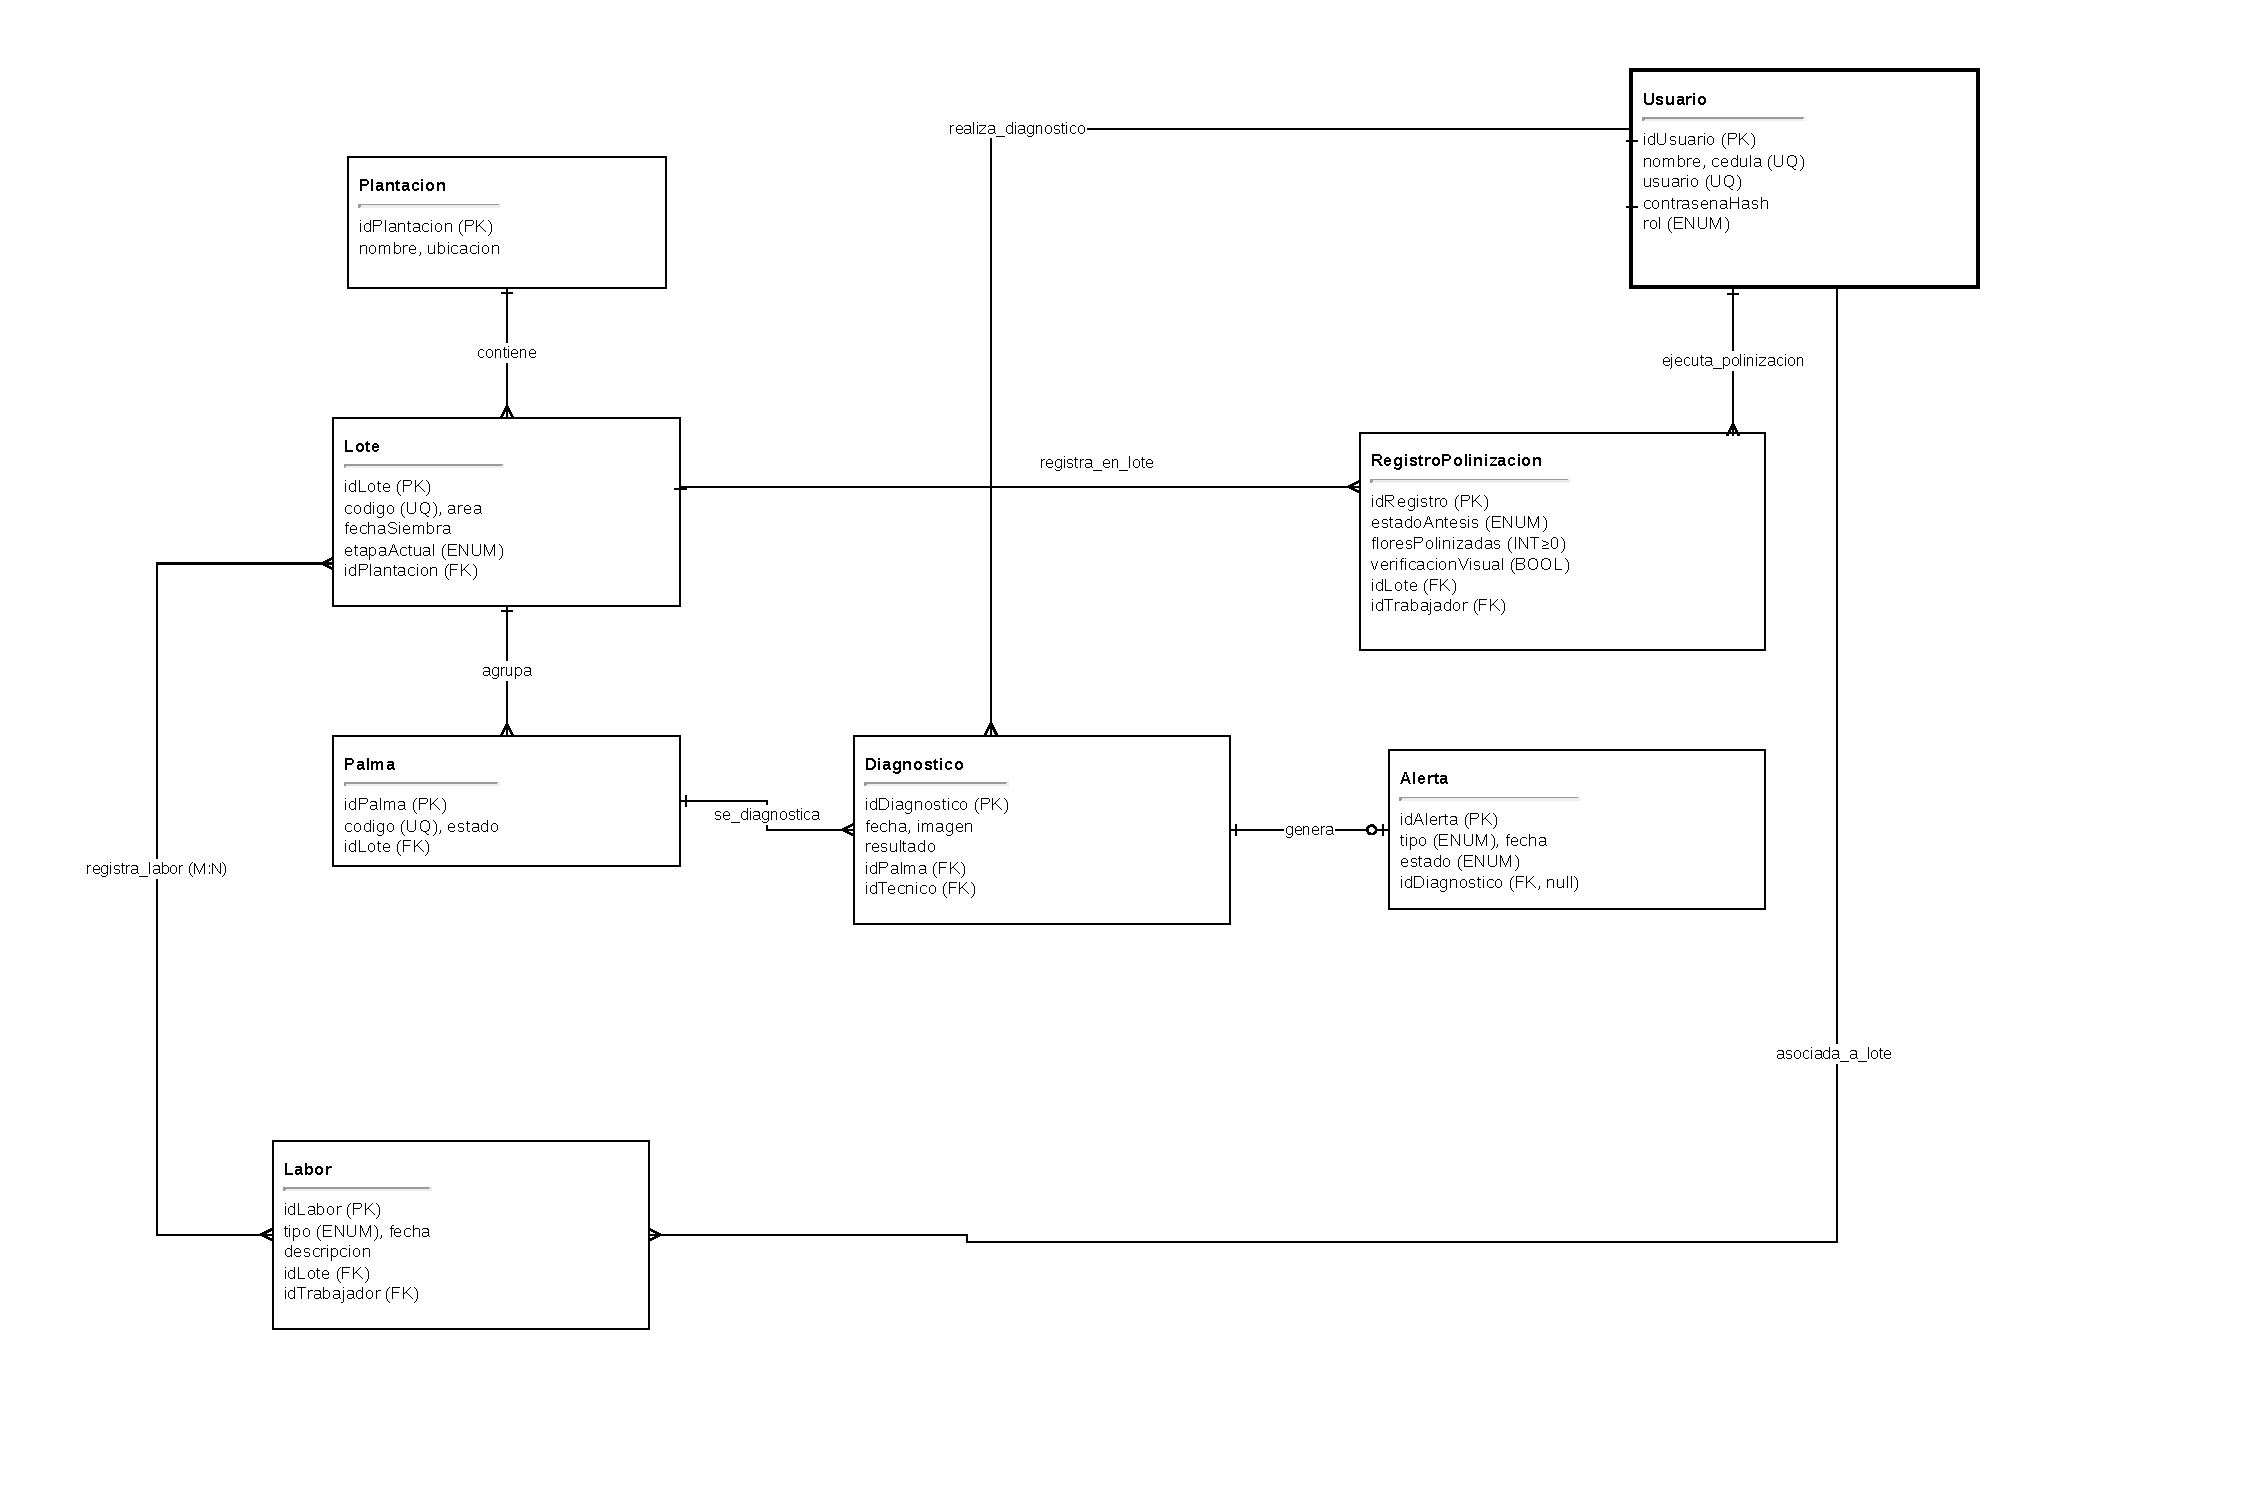
\includegraphics[width=\linewidth]{imagenes/Entidad-Relacion.drawio.pdf}
\caption{Diagrama entidad-relación del dominio SIMPA (notación Crow's Foot)}
\label{fig:diagrama-er}
\end{figure}

\section{Verificación de la Tercera Forma Normal (3FN)}

Se verificó que ninguna entidad presenta dependencias transitivas: todos los atributos no clave
dependen únicamente de la clave primaria completa de su entidad (2FN) y no existen atributos que
dependan de otro atributo no clave (3FN). Por ejemplo, en \textit{Diagnostico}, el atributo
\texttt{resultado} depende exclusivamente de \texttt{idDiagnostico} y no de \texttt{idPalma}, lo que
descarta una dependencia transitiva a través de la palma diagnosticada.

\section{Transformación al diagrama de clases UML}

El modelo ER se transformó en un diagrama de clases UML incorporando visibilidades, tipos de dato,
al menos dos operaciones por clase y una clase asociativa (\texttt{RegistroLaborTrabajador}) para
resolver la relación M:N \textit{registra\_labor}.

\begin{table}[H]
\centering
\caption{Operaciones principales de las clases UML (muestra)}
\label{tab:operaciones-clases}
\begin{tabularx}{\linewidth}{|l|Y|}
\hline
\textbf{Clase} & \textbf{Operaciones (visibilidad, firma)} \\
\hline
Diagnostico & +analizarImagen(imagen: Blob): ResultadoIA; +registrarDiagnostico(): void \\
\hline
Lote & +cambiarEtapa(nuevaEtapa: Etapa): void; +consultarHistorial(): List$\langle$Evento$\rangle$ \\
\hline
RegistroPolinizacion & +calcularConteoAutomatico(marcacionesGPS: List$\langle$Punto$\rangle$): int;
+registrarAntesis(estado: EstadoAntesis): void \\
\hline
Alerta & +generarAlerta(diagnostico: Diagnostico): void; +marcarAtendida(): void \\
\hline
\end{tabularx}
\end{table}

\begin{figure}[H]
\centering
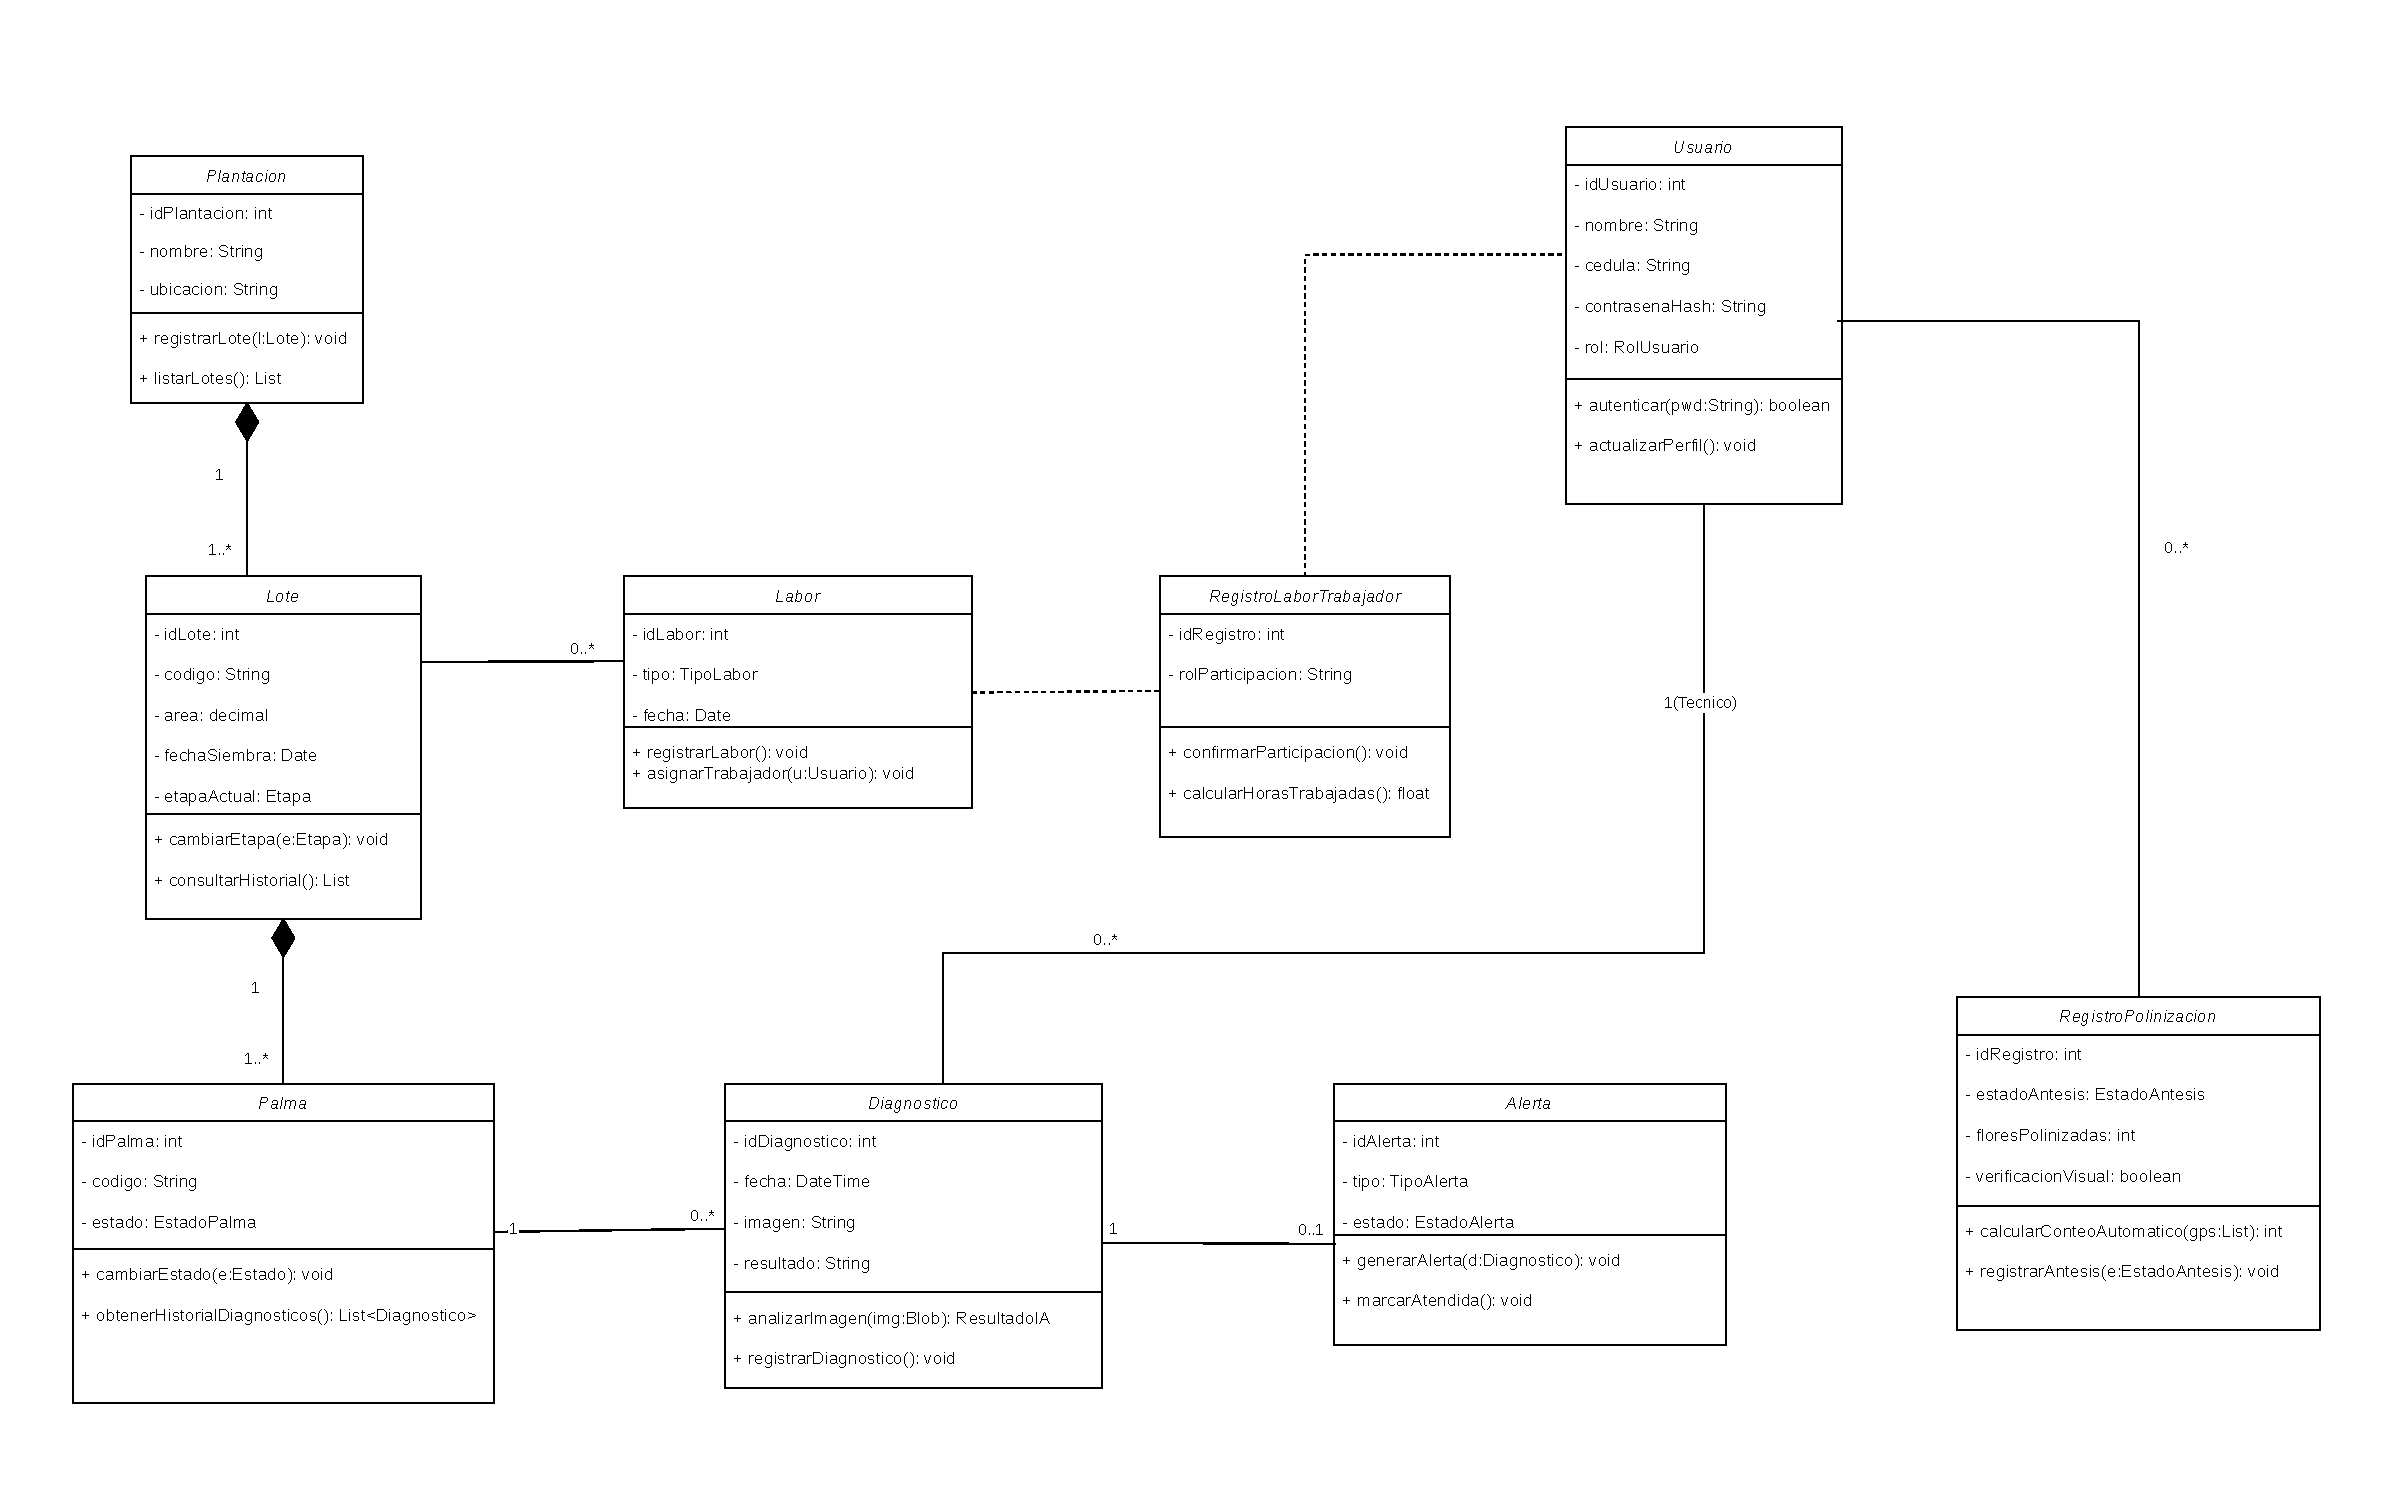
\includegraphics[width=\linewidth]{imagenes/Diagrama-Clases.drawio.pdf}
\caption{Diagrama de clases UML del dominio SIMPA}
\label{fig:diagrama-clases}
\end{figure}
\chapter{Modelo funcional: DFD y diagrama de actividades}

\section{Diagrama de contexto (DFD Nivel 0)}

El DFD de contexto representa al SIMPA como un proceso único que intercambia flujos de datos con las
cinco entidades externas ya identificadas en el diagrama de contexto de la Entrega 1B del PFC
(Administrador General, Técnico/Asesor, Trabajador/Polinizador, Dispositivo móvil GPS/cámara y
Estación meteorológica), añadiendo el servicio de IA y la base de conocimiento de plagas como
entidades externas adicionales requeridas por el modelo funcional.

\begin{table}[htbp]
\centering
\caption{Flujos de datos del DFD Nivel 0}
\label{tab:dfd0-flujos}
\begin{tabularx}{\linewidth}{|l|Y|}
\hline
\textbf{Entidad externa} & \textbf{Flujos de datos (entrada/salida)} \\
\hline
Administrador General & Gestiona cultivo, consulta reportes / Reportes, alertas, indicadores \\
\hline
Técnico/Asesor & Registra inspección, reporta plaga, registra análisis suelo-foliar / Diagnósticos,
recomendaciones \\
\hline
Trabajador/Polinizador & Registra labor, captura imagen, marcaciones GPS / Confirmación de registro \\
\hline
Servicio de análisis de IA & Imagen capturada / Resultado de clasificación (plaga, enfermedad,
deficiencia) \\
\hline
Estación meteorológica & Datos climáticos / -- \\
\hline
Base de conocimiento de plagas & Consulta especie/tratamiento / Ficha de plaga \\
\hline
\end{tabularx}
\end{table}

\begin{figure}[H]
\centering
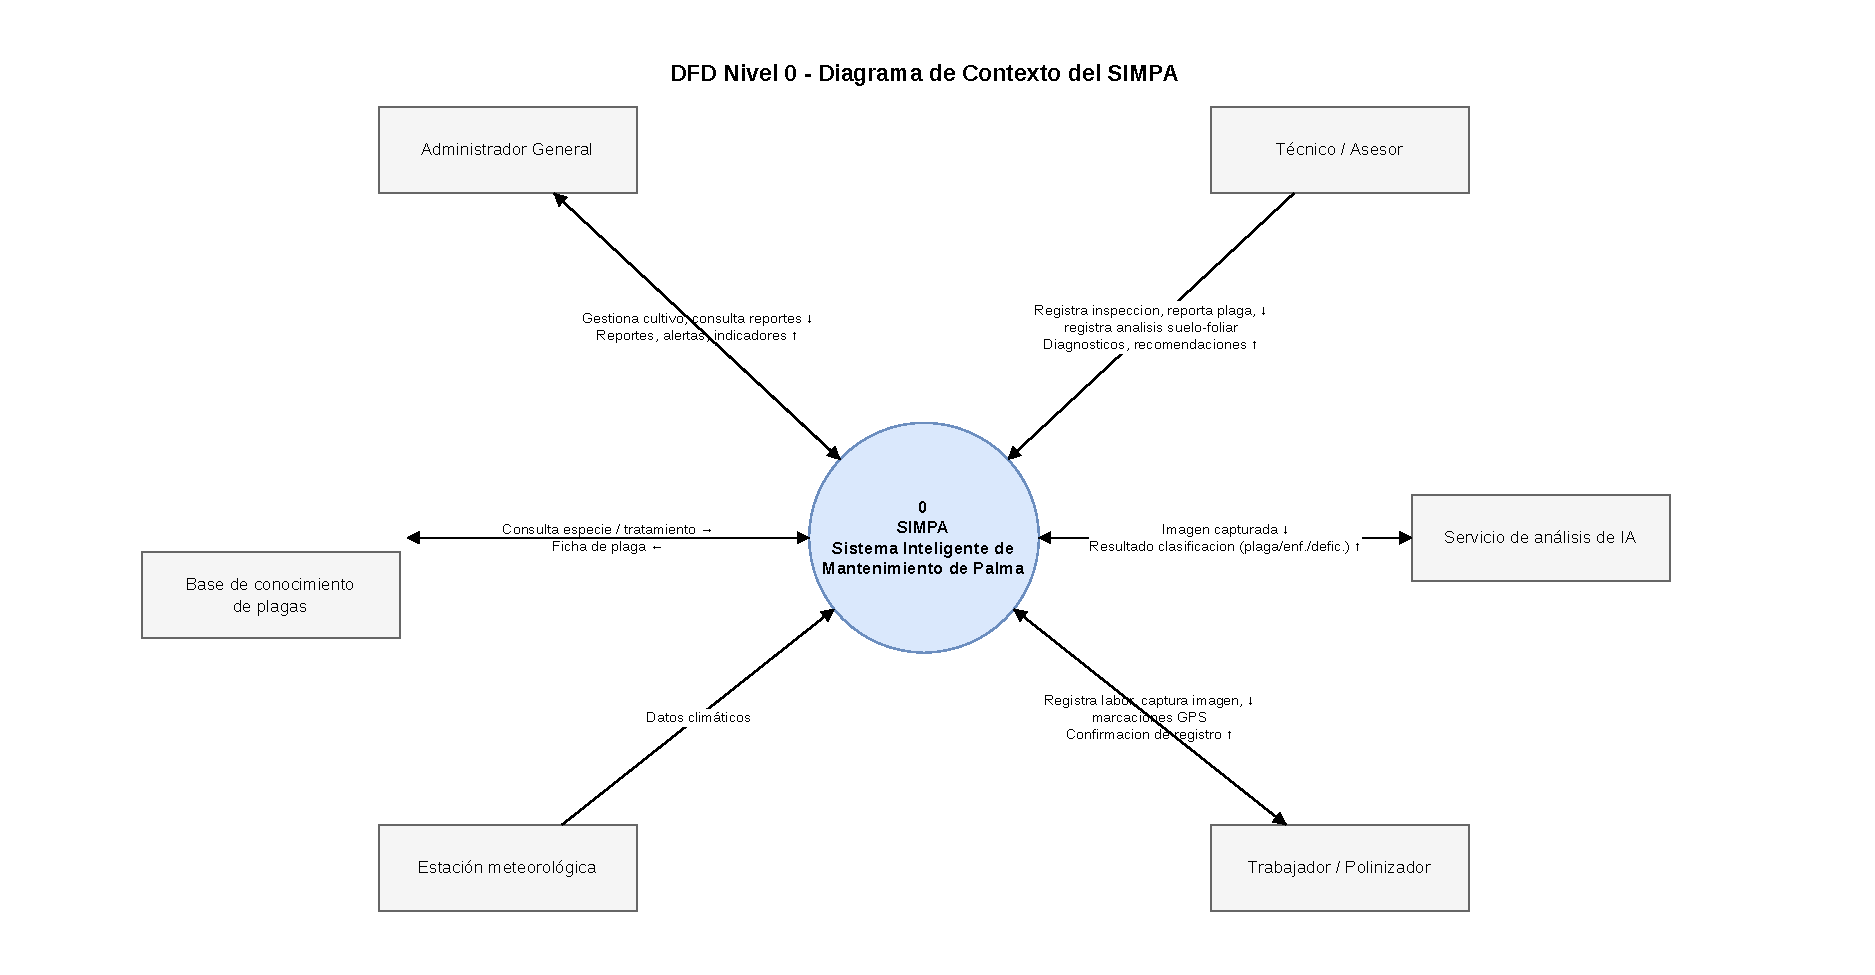
\includegraphics[width=\linewidth]{imagenes/Diagrama-DFD0.drawio.pdf}
\caption{DFD Nivel 0 -- Diagrama de contexto del SIMPA}
\label{fig:dfd-nivel0}
\end{figure}

\section{DFD Nivel 1}

El proceso central del Nivel 0 se descompuso en seis subprocesos con sus almacenes internos, verificando
el balanceo de flujos de entrada y salida respecto al Nivel 0.

\begin{table}[htbp]
\centering
\caption{Subprocesos y almacenes del DFD Nivel 1}
\label{tab:dfd1}
\begin{tabularx}{\linewidth}{|c|l|Y|}
\hline
\textbf{Proc.} & \textbf{Nombre} & \textbf{Almacenes internos relacionados} \\
\hline
P1 & Gestionar acceso y personal & D1 Usuarios, D2 Equipos \\
\hline
P2 & Gestionar lotes y plantaciones & D3 Lotes, D4 Plantaciones \\
\hline
P3 & Registrar labores y monitoreo & D5 Labores, D6 Monitoreos \\
\hline
P4 & Analizar imagen (IA) & D7 Diagnósticos \\
\hline
P5 & Registrar polinización y GPS & D8 RegistrosPolinizacion \\
\hline
P6 & Generar alertas y reportes & D9 Alertas, D10 Reportes \\
\hline
\end{tabularx}
\end{table}

\begin{figure}[H]
\centering
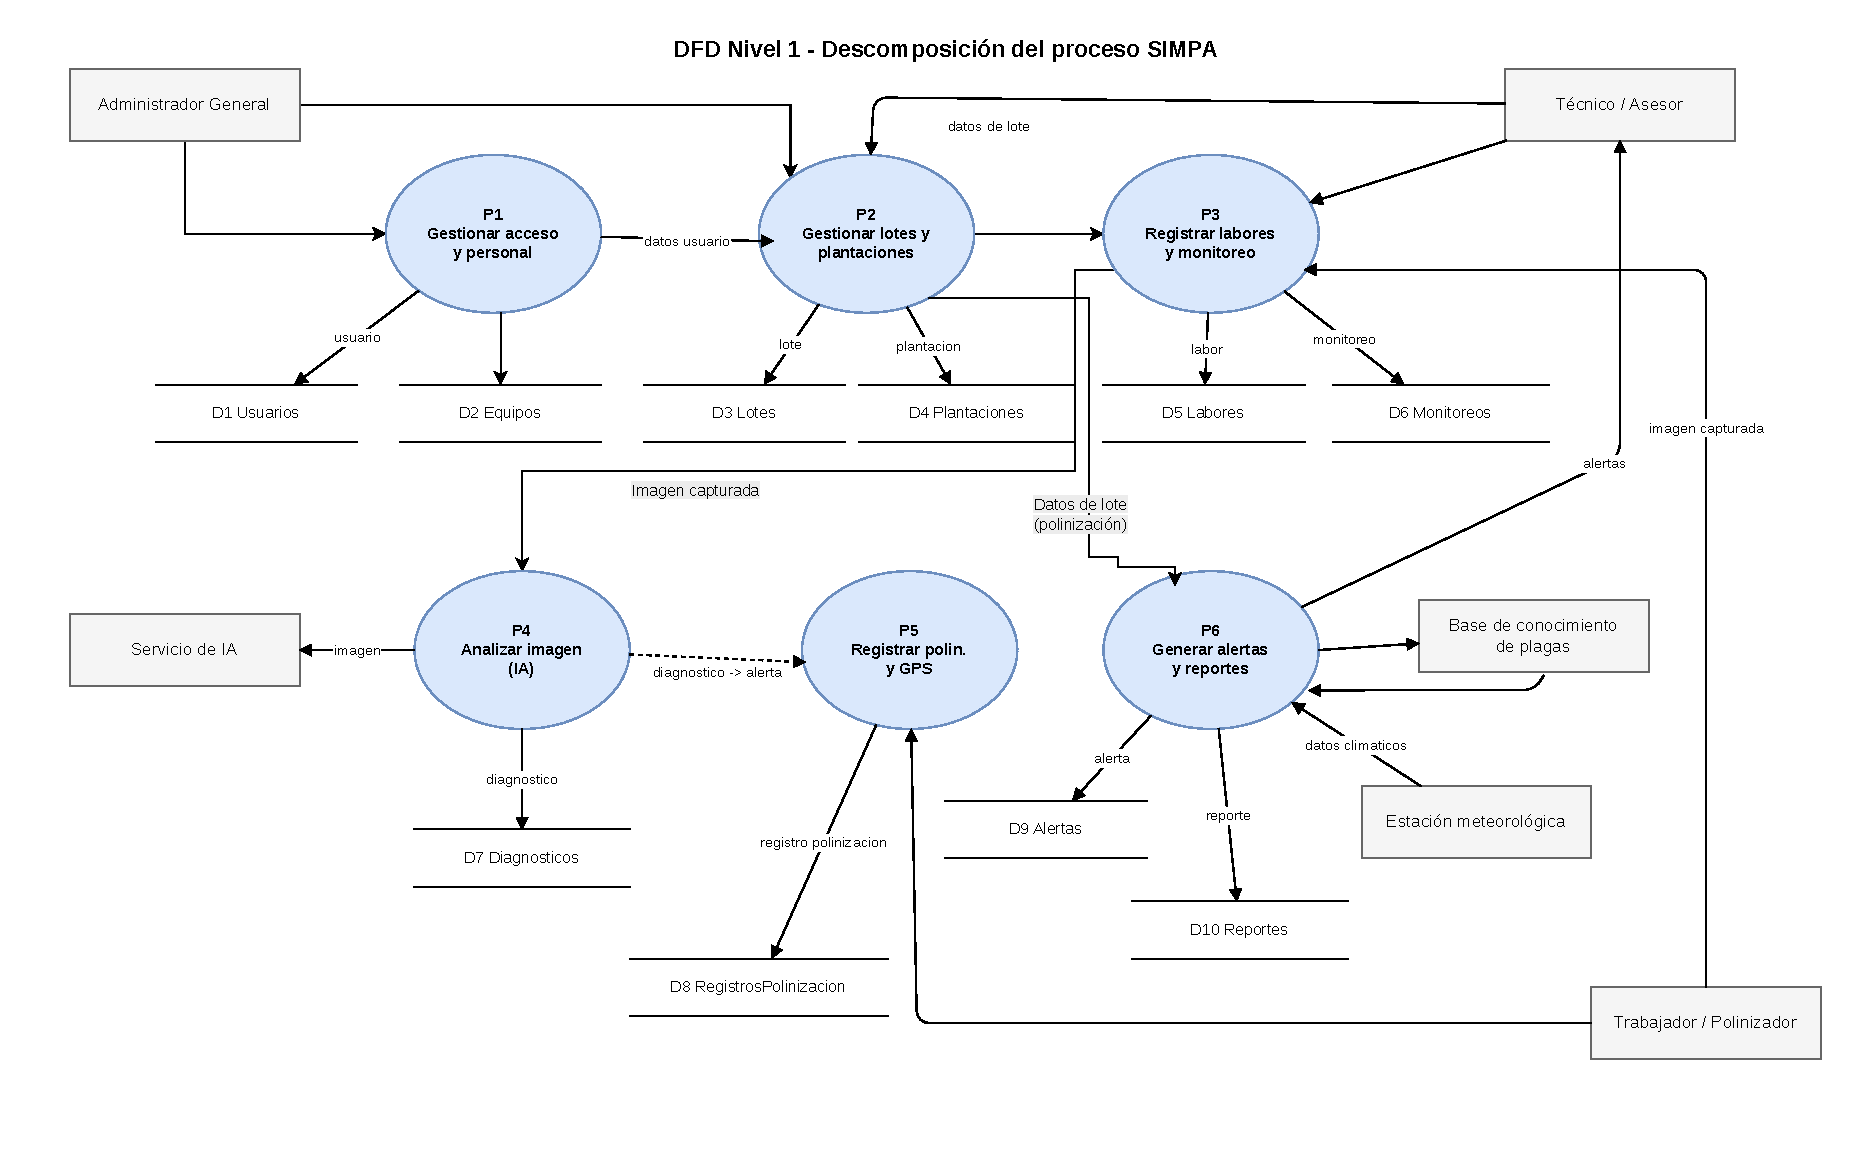
\includegraphics[width=\linewidth]{imagenes/Diagrama-DFD1.drawio.pdf}
\caption{DFD Nivel 1 -- Descomposición en subprocesos del SIMPA}
\label{fig:dfd-nivel1}
\end{figure}

\section{DFD esencial}

Se construyó el DFD esencial~\cite{maciaszek2007} para el proceso de negocio más importante del SIMPA:
la detección de plagas y enfermedades por imagen (RF-07/RF-08), separando la lógica esencial
(qué transformación de negocio ocurre) de la implementación tecnológica concreta (protocolo REST,
formato JSON, proveedor del modelo de IA).

\begin{figure}[H]
\centering
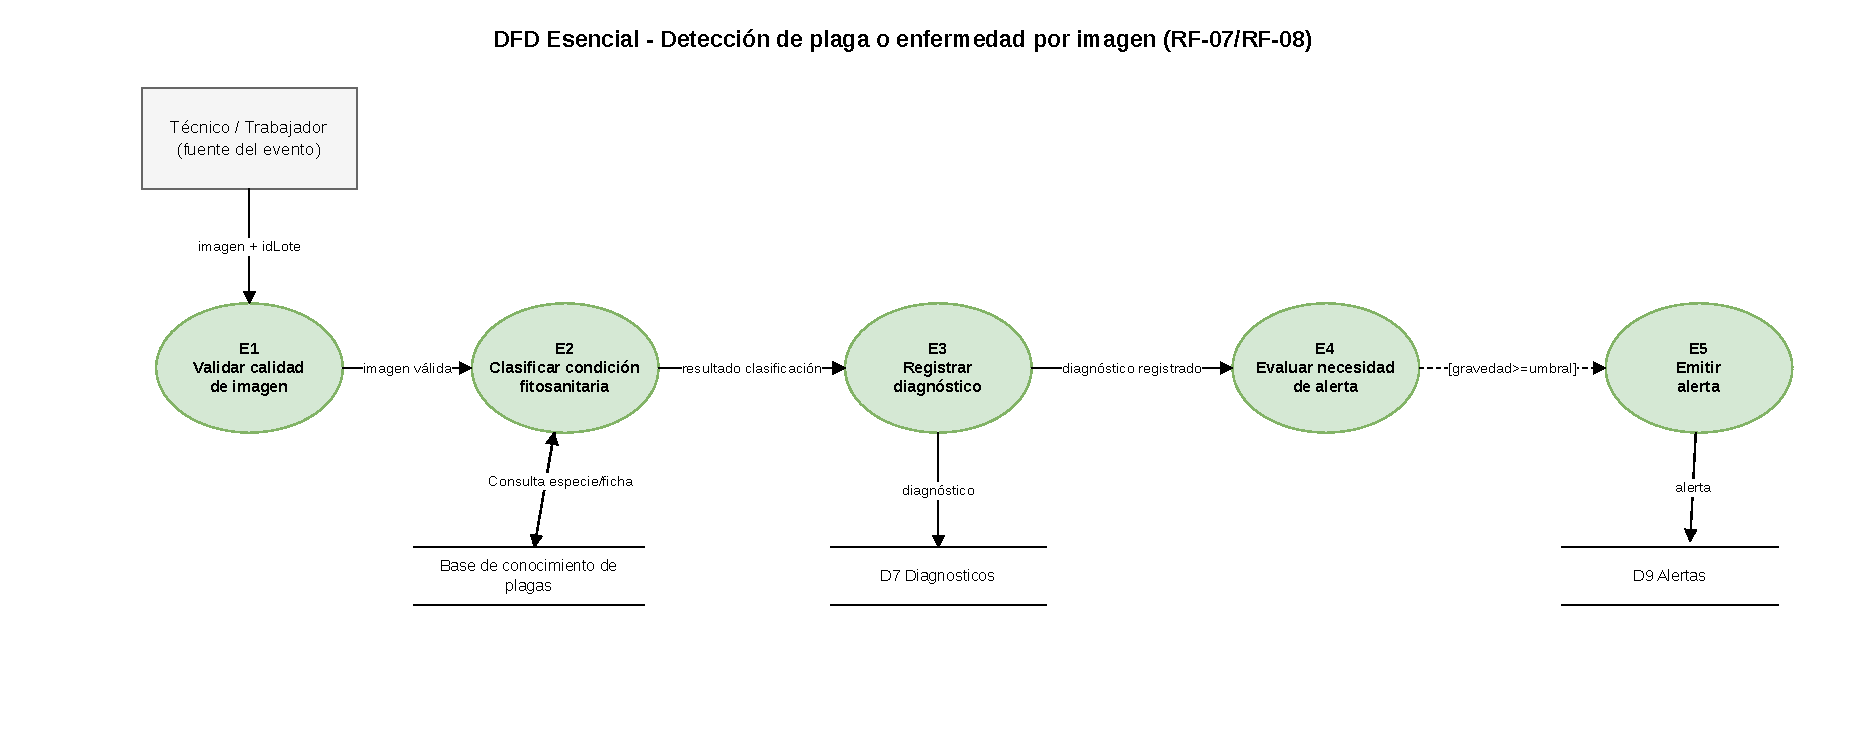
\includegraphics[width=\linewidth]{imagenes/Diagrama-DFDEsencial.drawio.pdf}
\caption{DFD esencial -- Detección de plaga o enfermedad por imagen (RF-07/RF-08)}
\label{fig:dfd-esencial}
\end{figure}

\section{Diagrama de actividades UML}

Se construyó el diagrama de actividades del caso de uso principal CU-01 (Analizar imagen para detectar
plaga o enfermedad), con swimlanes para el Técnico/Trabajador y el Servicio de análisis de IA, un nodo
de decisión sobre la calidad de la imagen, una bifurcación concurrente (fork/join) entre el
almacenamiento de la imagen y el envío al servicio de IA, y un flujo de objeto que transporta el
\textit{ResultadoIA} desde el servicio hasta el nodo de generación de alerta, conforme a las buenas
prácticas de modelado de comportamiento descritas por Pohl~\cite{pohl2025}.

\begin{figure}[H]
\centering
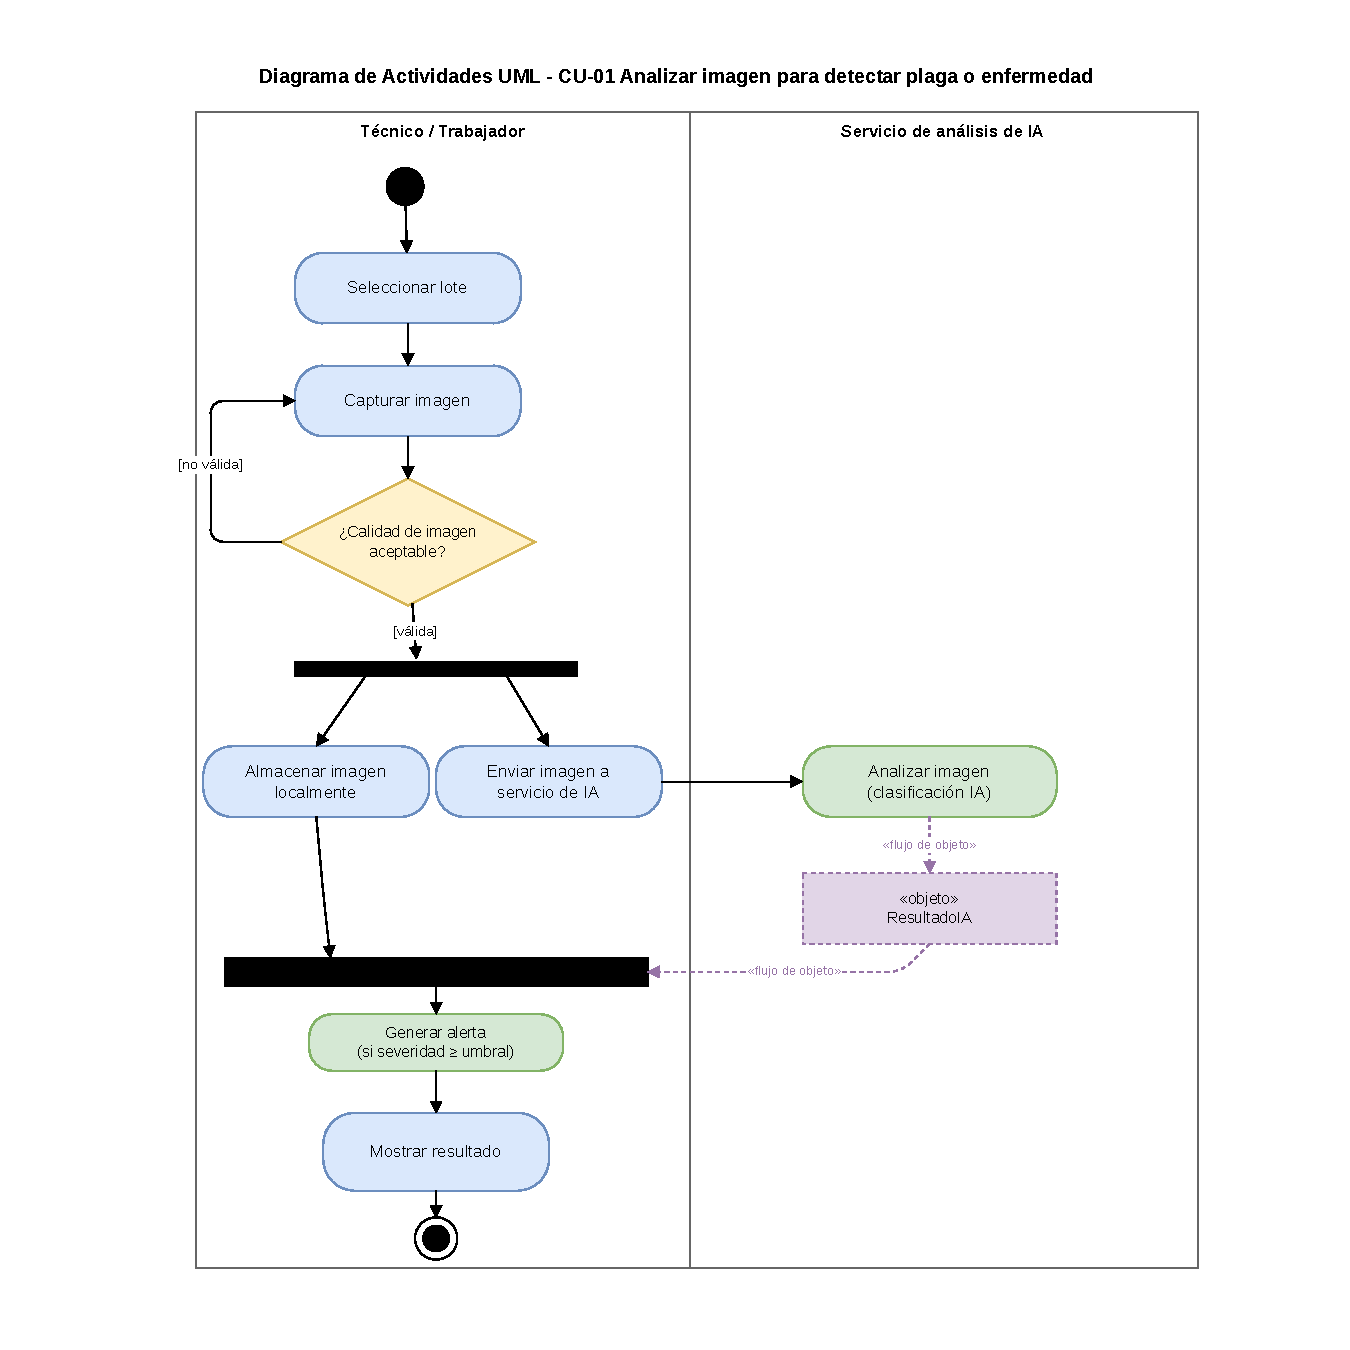
\includegraphics[width=\linewidth]{imagenes/Diagrama-Actividades.drawio.pdf}
\caption{Diagrama de actividades UML del caso de uso CU-01}
\label{fig:diagrama-actividades}
\end{figure}
\chapter{Modelo de comportamiento: máquina de estados y secuencia}

\section{Selección de la entidad}

Entre las entidades del dominio, \textit{Lote} es la que presenta el ciclo de vida más rico, con
cinco estados principales y un estado compuesto, por lo que se seleccionó para el modelado de
máquina de estados, siguiendo el formalismo de statecharts de Harel~\cite{harel1987}.

\section{Diagrama de máquina de estados}

\begin{table}[H]
\centering
\caption{Estados, eventos y acciones del ciclo de vida de Lote}
\label{tab:estados}
\begin{tabularx}{\linewidth}{|>{\hsize=0.6\hsize}X|>{\hsize=1.2\hsize}X|>{\hsize=1.2\hsize}X|}
\hline
\textbf{Estado} & \textbf{Evento de entrada [condición]} & \textbf{Acción} \\
\hline
Sembrado & registrarLote() & inicializarEtapaActual('Sembrado') \\
\hline
\multirow{2}{*}{EnCrecimiento} & \multirow{2}{*}{tiempoTranscurrido [$\geq$ 12 meses]} & \multirow{2}{*}{actualizarEtapa('EnCrecimiento')} \\
(compuesto: \{Vegetativo, PreAntesis\}) & & \\
\hline
EnPolinizacion & antesisDetectada() & habilitarRegistroPolinizacion() \\
\hline
EnFructificacion & polinizacionCompletada() [floresPolinizadas $>$ 0] & iniciarSeguimientoRacimo() \\
\hline
ListoParaCosecha & censoFlores() [rendimientoEstimado $\geq$ umbral] & generarAlertaCosecha() \\
\hline
Cosechado & registrarCosecha() & cerrarCicloProductivo() \\
\hline
\end{tabularx}
\end{table}

El estado \textit{EnCrecimiento} se modela como estado compuesto con dos subestados
(\textit{Vegetativo} y \textit{PreAntesis}), reflejando que durante el crecimiento el lote puede
recibir análisis de suelo y foliar sin que ello constituya un cambio de etapa principal.

\begin{figure}[H]
\centering
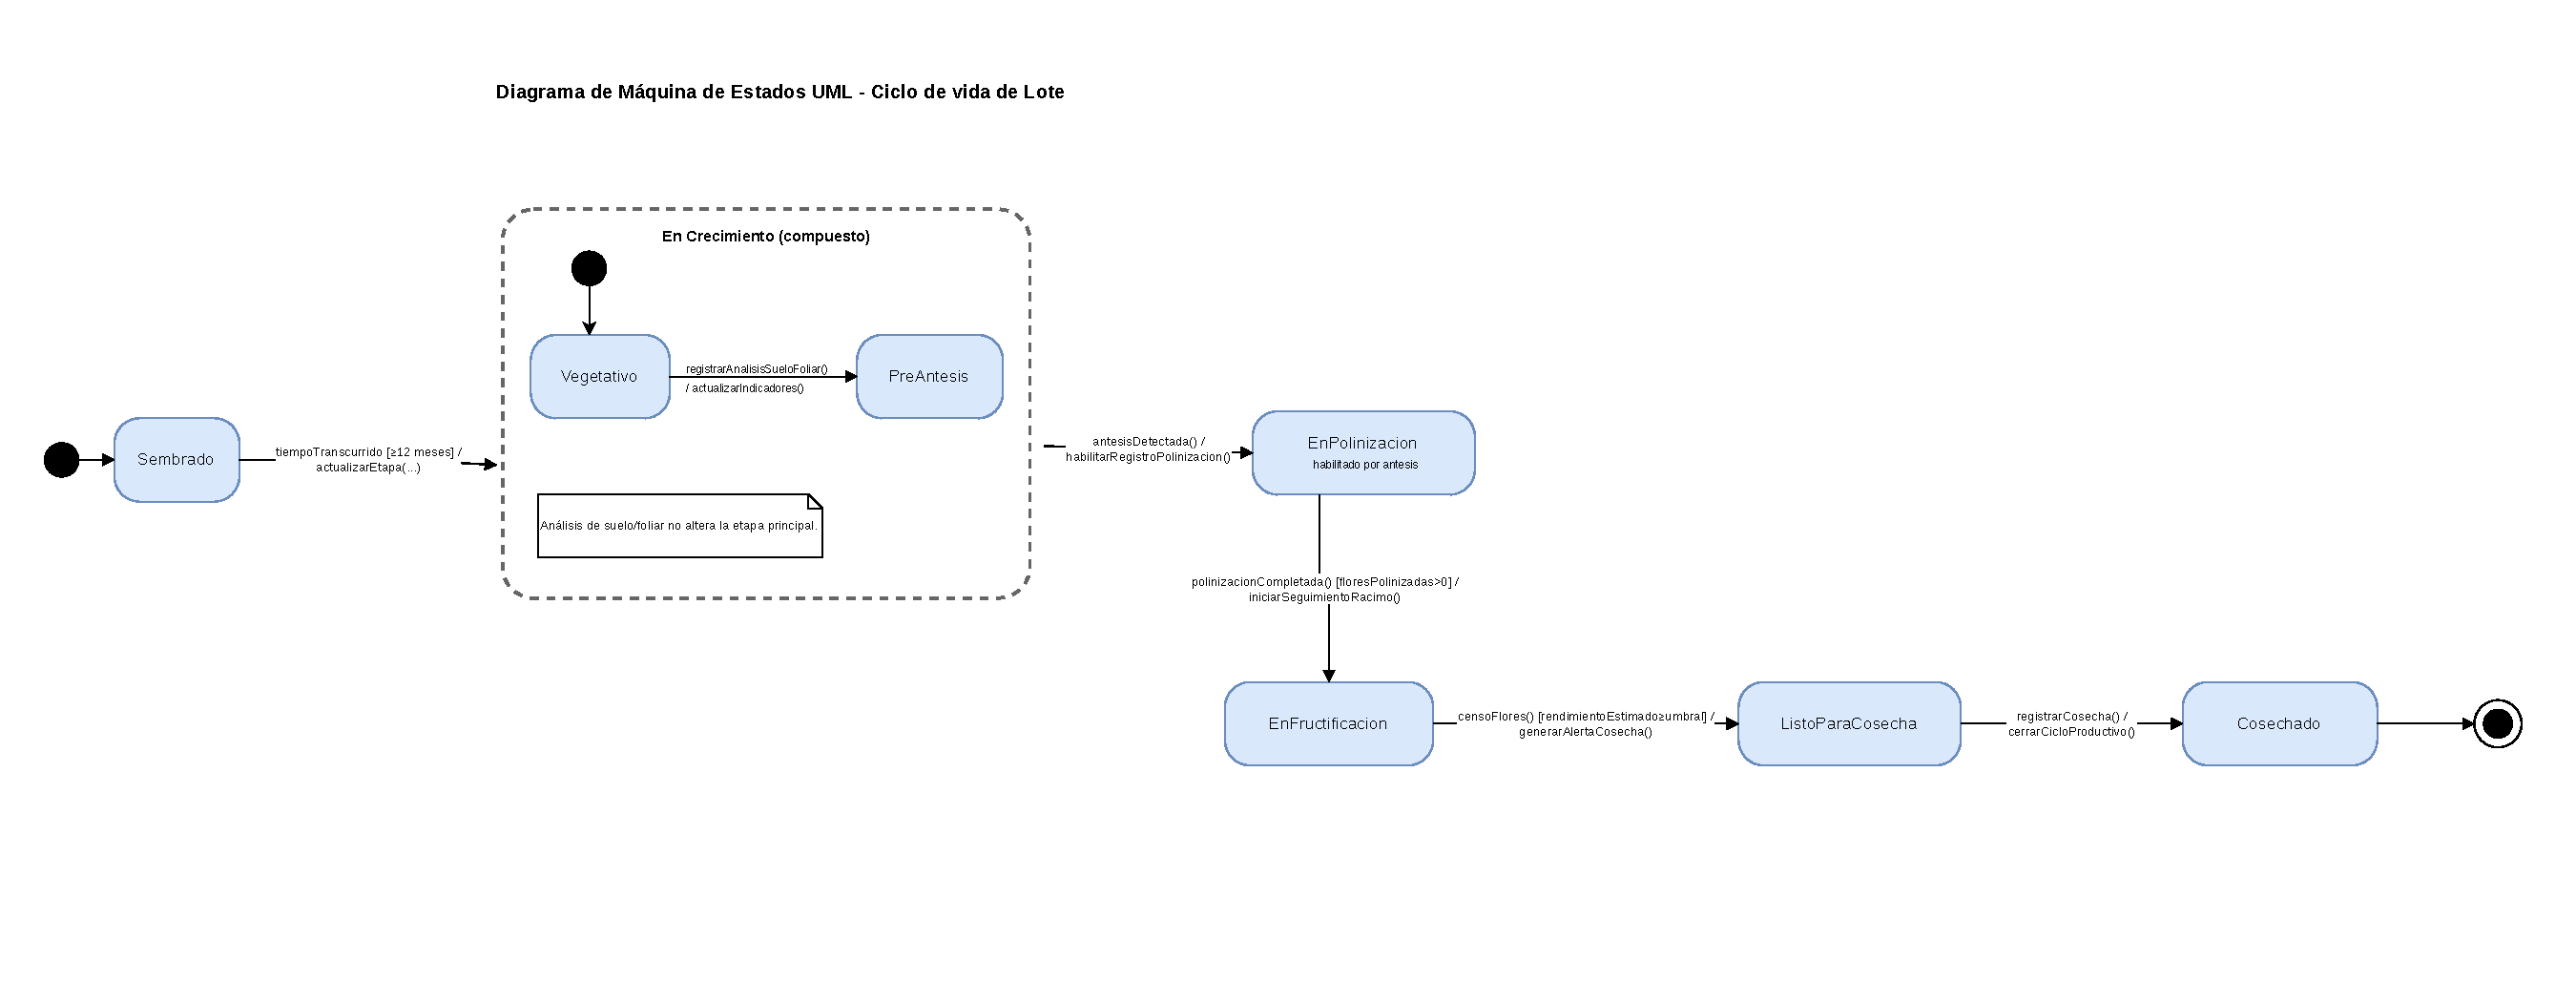
\includegraphics[width=\linewidth]{imagenes/Diagrama-Estados.drawio.pdf}
\caption{Diagrama de máquina de estados UML del ciclo de vida de Lote}
\label{fig:diagrama-estados}
\end{figure}

\section{Diagrama de secuencia}

Se construyó el diagrama de secuencia UML del escenario principal del caso de uso CU-01 (Analizar
imagen para detectar plaga o enfermedad), con cinco líneas de vida: \textit{Técnico/Trabajador},
\textit{AppMóvil}, \textit{APIREST}, \textit{ServicioIA} y \textit{BaseDeDatos}. El diagrama incluye
un fragmento \texttt{alt} para diferenciar la respuesta según la calidad de la imagen (válida/no
válida) y un fragmento \texttt{loop} para el reintento de captura cuando la imagen es rechazada.

\begin{enumerate}[label=\arabic*.]
\item Técnico/Trabajador $\rightarrow$ AppMóvil: seleccionarLote(); capturarImagen()
\item AppMóvil $\rightarrow$ APIREST: enviarImagen(imagen, idLote)
\item \texttt{alt} [imagen válida]
  \begin{itemize}
    \item APIREST $\rightarrow$ ServicioIA: analizarImagen(imagen)
    \item ServicioIA $\rightarrow$ APIREST: resultadoIA(diagnostico)
    \item APIREST $\rightarrow$ BaseDeDatos: guardarDiagnostico(diagnostico)
    \item APIREST $\rightarrow$ AppMóvil: mostrarResultado(diagnostico)
  \end{itemize}
\item \texttt{alt} [imagen no válida] \texttt{loop} [hasta 3 intentos]
  \begin{itemize}
    \item APIREST $\rightarrow$ AppMóvil: solicitarNuevaCaptura()
  \end{itemize}
\end{enumerate}

\begin{figure}[H]
\centering
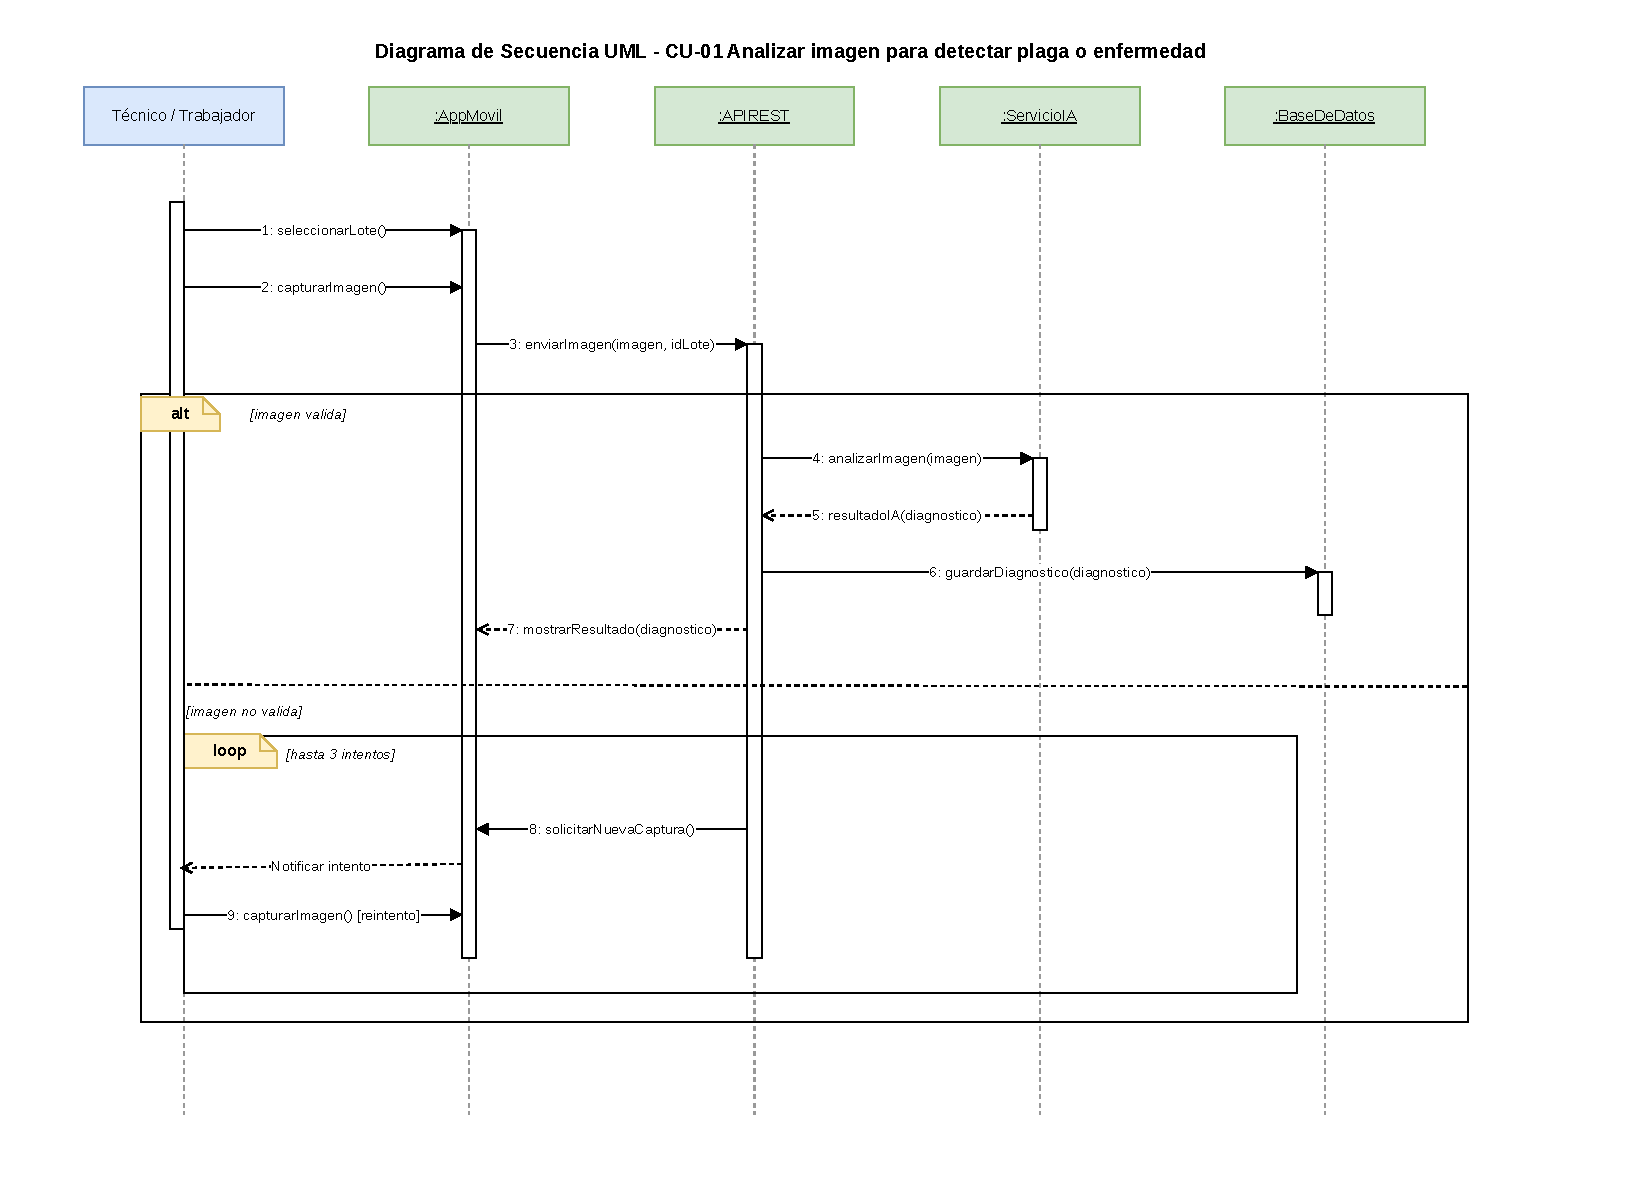
\includegraphics[width=\linewidth]{imagenes/Diagrama-Secuencia.drawio.pdf}
\caption{Diagrama de secuencia UML del caso de uso CU-01}
\label{fig:diagrama-secuencia}
\end{figure}
\chapter{Matriz de trazabilidad y tabla comparativa}
\label{sec:trazabilidad}

\section{Matriz de trazabilidad}

La matriz de trazabilidad enlaza cada requisito funcional con los casos de uso, las clases UML, los
procesos del DFD, las actividades y los estados en los que se manifiesta, siguiendo el requisito de
trazabilidad bidireccional de IEEE/ISO/IEC 15288:2023~\cite{ieee15288}.

\begin{landscape}
\begin{table}[htbp]
\centering
\footnotesize
\caption{Matriz de trazabilidad RF vs. modelos UML/DFD}
\label{tab:matriz-trazabilidad}
\begin{tabularx}{\linewidth}{|>{\hsize=0.5\hsize}X|>{\hsize=1.0\hsize}X|>{\hsize=1.0\hsize}X|>{\hsize=0.7\hsize}X|>{\hsize=0.7\hsize}X|>{\hsize=1.1\hsize}X|}
\hline
\textbf{RF} & \textbf{Caso de uso} & \textbf{Clase(s) UML} & \textbf{Proceso DFD} & \textbf{Actividad} & \textbf{Estado} \\
\hline
RF-01 & Iniciar sesión & Usuario & P1 & -- & -- \\
RF-02 & Gestionar lotes & Lote, Plantacion & P2 & -- & Sembrado \\
RF-03 & Gestionar personal & Usuario & P1 & -- & -- \\
RF-04 & Registrar labor & Labor, RegistroLaborTrabajador & P3 & Nodo "Registrar labor" & -- \\
RF-05 & Registrar monitoreo & Diagnostico & P3 & -- & -- \\
RF-06 & Detalle de lote & Lote & P2 & -- & EnCrecimiento/EnPolinizacion \\
RF-07 & Analizar imagen & Diagnostico, Palma & P4 & Todo CU-01 & -- \\
RF-08 & Diagnóstico nutricional & Diagnostico, Palma & P4 & Similar a CU-01 & -- \\
RF-09 & Recomendar control & Diagnostico & P4 & Nodo "Recomendar control" & -- \\
RF-10 & Gestionar variedades & Lote, Palma & P2 & -- & -- \\
RF-11 & Registrar análisis & Diagnostico & P3 & -- & -- \\
RF-12 & Generar alerta & Alerta & P6 & Nodo join $\rightarrow$ Alerta & -- \\
RF-13 & Registrar polinización & RegistroPolinizacion & P5 & Todo CU-03 & EnPolinizacion \\
RF-14 & Conteo por GPS & RegistroPolinizacion & P5 & Nodo "Calcular conteo" & -- \\
RF-15 & Monitorear recorridos & RegistroPolinizacion & P5 & -- & -- \\
RF-16 & Evaluar desempeño & Usuario, Labor & P6 & -- & -- \\
RF-17 & Registrar/consultar clima & -- (externo) & P6 & -- & -- \\
RF-18 & Estimar producción & Lote & P6 & -- & ListoParaCosecha \\
RF-19 & Generar reporte & Reporte & P6 & Todo CU-05 & -- \\
RF-20 & Consultar historial & Diagnostico, Labor & P6 & -- & -- \\
\hline
\end{tabularx}
\end{table}
\end{landscape}

\subsection{Análisis de cobertura}

De la matriz anterior se observa que todos los requisitos funcionales (RF-01 a RF-20) cuentan con al
menos un caso de uso, una clase UML y un proceso DFD asociado, por lo que no se identifican requisitos
sin cobertura (\textit{gaps}). Sin embargo, tres procesos del DFD Nivel 1 (P1, P2, P6) agrupan
varios requisitos sin una actividad UML dedicada, lo cual es consistente con su naturaleza
transaccional (alta cohesión de tipo CRUD) y no constituye sobreespecificación. No se detectaron
modelos --clases, procesos o estados-- sin ningún requisito funcional asociado, por lo que tampoco se
identifican casos de \textit{gold plating}~\cite{ieee29148}.

\section{Tabla comparativa de las tres perspectivas de modelado}

\begin{table}[htbp]
\centering
\caption{Comparación de las perspectivas de datos, funcional y de comportamiento}
\label{tab:comparativa}
\begin{tabularx}{\linewidth}{|>{\hsize=0.8\hsize}X|>{\hsize=1.1\hsize}X|>{\hsize=1.1\hsize}X|>{\hsize=1.0\hsize}X|}
\hline
\multicolumn{1}{|c|}{\textbf{Criterio}} & 
\multicolumn{1}{c|}{\textbf{Datos}} & 
\multicolumn{1}{c|}{\textbf{Funcional}} & 
\multicolumn{1}{c|}{\textbf{Comportamiento}} \\
\multicolumn{1}{|c|}{} & 
\multicolumn{1}{c|}{\textbf{(ER/Clases)}} & 
\multicolumn{1}{c|}{\textbf{(DFD/Actividades)}} & 
\multicolumn{1}{c|}{\textbf{(Estados/Secuencia)}} \\
\hline
Perspectiva cubierta & Estructura estática de la información y sus relaciones. & Transformación de datos por procesos y su descomposición jerárquica. & Evolución temporal de una entidad y orden de interacción entre objetos. \\
\hline
Notación & Entidad-relación (Crow's Foot) y clases UML. & DFD (Yourdon/Gane-Sarson) y actividades UML. & Statecharts de Harel~\cite{harel1987} y secuencia UML. \\
\hline
Requisitos que ayuda a descubrir & Atributos faltantes, entidades implícitas, relaciones M:N no declaradas (p.ej., RF-02, RF-10). & Procesos huérfanos, flujos de datos no balanceados, RF de generación de reportes (RF-19). & Transiciones no contempladas, condiciones de guarda ausentes, RF de polinización (RF-13, RF-14). \\
\hline
Limitaciones & No expresa el orden temporal ni las condiciones de activación de los procesos. & No captura el ciclo de vida completo de una única entidad ni las condiciones de guarda entre estados. & No representa por sí sola la estructura completa de datos ni la descomposición jerárquica de procesos. \\
\hline
\end{tabularx}
\end{table}

\chapter{Conclusiones}

\begin{enumerate}[label=\arabic*.]

\item La revisión del SRS parcial de la Entrega 1B del SIMPA, contrastada contra los criterios de
calidad de IEEE/ISO/IEC 29148:2018~\cite{ieee29148}, permitió identificar seis defectos concretos
--principalmente de ambigüedad y verificabilidad--, cuya corrección mediante la sintaxis
EARS~\cite{mavin2009} incrementó la precisión operacional de los requisitos sin alterar su alcance
funcional original.

\item El modelo de datos, compuesto por ocho entidades y nueve relaciones --incluidas dos relaciones
muchos a muchos--, resultó consistente con el diagrama de clases conceptual de dieciocho clases
construido en la Entrega 1B, confirmando que la perspectiva de datos del SIMPA está suficientemente
estabilizada para avanzar hacia el diseño detallado.

\item El modelo funcional, expresado en tres niveles de DFD y un diagrama de actividades, evidenció
que el proceso de análisis de imagen por inteligencia artificial (RF-07/RF-08) es el núcleo
transformador del sistema, lo cual es coherente con su clasificación \textit{Must} en la priorización
MoSCoW de la Entrega 1B y con la evidencia empírica reportada en la literatura reciente sobre
clasificación de enfermedades de palma mediante redes convolucionales~\cite{abuzanona2022,hamdani2021}.

\item El modelo de comportamiento reveló que la entidad \textit{Lote} concentra la mayor complejidad
de estados del dominio, y que el escenario de análisis de imagen (CU-01) requiere fragmentos
condicionales (\texttt{alt}) y de repetición (\texttt{loop}) para representar adecuadamente los
casos de imagen rechazada, un detalle no explícito en la especificación textual original.

\item La matriz de trazabilidad de veinte requisitos funcionales frente a los modelos de datos,
funcionales y de comportamiento no reveló requisitos sin cobertura ni artefactos de modelado sin
respaldo en un requisito, lo que confirma la completitud del conjunto de modelos entregado en esta
práctica y su alineación con los principios de trazabilidad de IEEE/ISO/IEC 15288:2023~\cite{ieee15288}.

\end{enumerate}

Como trabajo futuro se recomienda profundizar la validación empírica de los requisitos no funcionales
de desempeño de la inteligencia artificial (NFR-02) mediante pruebas de campo con conectividad real,
apoyándose en arquitecturas de IoT agrícola ya documentadas en la literatura~\cite{chamara2022}, y
extender el diagrama de máquina de estados a la entidad \textit{Diagnostico} para modelar de forma
explícita su ciclo de revisión y cierre por parte del técnico responsable.

\clearpage
\bibliographystyle{ieeetr}
\bibliography{referencias}

\appendix
\chapter{Tabla de atributos completa de todos los RF y RNF}

\begin{longtable}{|
p{1.2cm}|
p{4.4cm}|
p{0.8cm}|
p{1.7cm}|
p{1.3cm}|
p{2cm}|
p{1.5cm}|
p{0.8cm}|}
\hline
\textbf{ID} & \textbf{Descripción} & \textbf{Tipo} & \textbf{MoSCoW} & \textbf{Fuente} &
\textbf{Estabilidad} & \textbf{Estado} & \textbf{Verif.} \\
\hline
\endfirsthead
\hline
\textbf{ID} & \textbf{Descripción} & \textbf{Tipo} & \textbf{MoSCoW} & \textbf{Fuente} &
\textbf{Estabilidad} & \textbf{Estado} & \textbf{Verif.} \\
\hline
\endhead
RF-01 & Autenticación y control de acceso por rol & RF & Must & EV-01, EV-04 & Estable & Aprobado & S \\ \hline
RF-02 & Gestión de plantaciones y lotes & RF & Must & EV-01, EV-02, EV-04 & Estable & Aprobado & S \\ \hline
RF-03 & Gestión de personal y equipos de trabajo & RF & Must & EV-01 & Estable & Aprobado & S \\ \hline
RF-04 & Registro de labores agrícolas & RF & Must & EV-01, EV-02, EV-03 & Estable & Aprobado & S \\ \hline
RF-05 & Registro de monitoreo fitosanitario diario & RF & Must & EV-01, EV-02, EV-04 & Estable & Aprobado & S \\ \hline
RF-06 & Seguimiento de etapas del cultivo & RF & Should & EV-01 & Estable & Aprobado & S \\ \hline
RF-07 & Detección de plagas y enfermedades por imagen (IA) & RF & Must & EV-01, EV-02 & Volátil & Aprobado & S \\ \hline
RF-08 & Diagnóstico de deficiencias nutricionales por imagen (IA) & RF & Must & EV-02 & Volátil & Aprobado & S \\ \hline
RF-09 & Ficha de plaga: especie, ciclo y recomendación de control & RF & Should & EV-01, EV-02 & Volátil & Aprobado & S \\ \hline
RF-10 & Gestión de variedades de palma & RF & Could & EV-01, EV-02 & Estable & Aprobado & S \\ \hline
RF-11 & Registro de análisis de suelo y foliar & RF & Should & EV-02 & Estable & Aprobado & S \\ \hline
RF-12 & Generación de alertas tempranas & RF & Must & EV-01, EV-02 & Estable & Aprobado & S \\ \hline
RF-13 & Registro del proceso de polinización & RF & Must & EV-03 & Estable & Aprobado & S \\ \hline
RF-14 & Conteo automático de flores polinizadas por GPS & RF & Must & EV-03 & Volátil & Aprobado & S \\ \hline
RF-15 & Registro y monitoreo de recorridos del personal (GPS) & RF & Should & EV-01, EV-02, EV-03 & Estable & Aprobado & S \\ \hline
RF-16 & Evaluación de desempeño del personal & RF & Should & EV-01, EV-02, EV-03 & Estable & Aprobado & S \\ \hline
RF-17 & Registro y consulta de datos climáticos & RF & Should & EV-01, EV-02, EV-03 & Estable & Aprobado & S \\ \hline
RF-18 & Estimación de producción y rendimiento & RF & Must & EV-01, EV-02 & Volátil & Aprobado & S \\ \hline
RF-19 & Generación de reportes & RF & Must & EV-01, EV-02 & Estable & Aprobado & S \\ \hline
RF-20 & Historial de actividades, diagnósticos y eventos & RF & Should & EV-01 & Estable & Aprobado & S \\ \hline
NFR-01 & Eficiencia de desempeño ($\leq$ 3 s, 50 usuarios concurrentes) & RNF & Should & Derivado & Estable & Aprobado & S \\ \hline
NFR-02 & Eficiencia de desempeño de la IA ($\leq$ 10 s, P95) & RNF & Must & EV-01, EV-02 & Volátil & Aprobado & S \\ \hline
NFR-03 & Disponibilidad del backend $\geq$ 99\% mensual & RNF & Should & Derivado & Estable & Aprobado & S \\ \hline
NFR-04 & Operación offline con sincronización sin pérdida & RNF & Must & EV-01 & Estable & Aprobado & S \\ \hline
NFR-05 & Usabilidad para usuarios sin experiencia previa & RNF & Must & EV-01, EV-02 & Estable & Aprobado & S \\ \hline
NFR-06 & Seguridad: hash de contraseñas y TLS 1.2+ & RNF & Must & Derivado & Estable & Aprobado & S \\ \hline
NFR-07 & Compatibilidad Android 9.0+ y navegadores recientes & RNF & Should & Derivado & Estable & Aprobado & S \\ \hline
NFR-08 & Precisión GPS $\leq$ 10 m, muestreo $\leq$ 30 s & RNF & Should & EV-03 & Estable & Aprobado & S \\ \hline
NFR-09 & Cobertura de pruebas $\geq$ 60\% & RNF & Could & Derivado & Volátil & Aprobado & S \\ \hline
\end{longtable}


\chapter{Registro de defectos del SRS con correcciones aplicadas}

\begin{longtable}{|c|p{4cm}|c|p{5.5cm}|}
\hline
\textbf{ID} & \textbf{Defecto} & \textbf{Tipo} & \textbf{Corrección aplicada (EARS)} \\
\hline
\endfirsthead
\hline
\textbf{ID} & \textbf{Defecto} & \textbf{Tipo} & \textbf{Corrección aplicada (EARS)} \\
\hline
\endhead
D-01 & RF-04 mezcla varios subtipos de labor en un único enunciado & Ambigüedad / no singular &
\textit{While} the user is authenticated and the lot exists, the SIMPA \textit{shall} allow the
registration of a labor of type irrigation, pollination, phytosanitary control, or maintenance. \\
\hline
D-02 & RF-06 no especifica el evento disparador del cambio de etapa & No verificable & \textit{When}
the administrator registers a stage change for a lot, the SIMPA \textit{shall} update the lot's
current stage and log the transition. \\
\hline
D-03 & RF-09 no declara explícitamente su precondición en el enunciado & Incompletitud &
\textit{While} a pest diagnosis exists for a lot, the SIMPA \textit{shall} display species, life
cycle, and recommended control action. \\
\hline
D-04 & NFR-02 no indica percentil de medición del tiempo de respuesta & No verificable & \textit{While}
bandwidth is at least 5 Mbps, the SIMPA \textit{shall} return a diagnosis within 10 seconds for at
least the 95th percentile of requests. \\
\hline
D-05 & RF-14 usa lenguaje impreciso sobre el mecanismo de conteo & Ambigüedad & \textit{While} GPS
tracking is active with sampling $\leq$ 30 s, the SIMPA \textit{shall} compute automatically the
daily pollinated-flower count per worker. \\
\hline
D-06 & RD-05 no está trazada a ningún NFR de disponibilidad & Trazabilidad incompleta & Se añadió la
traza RD-05 $\rightarrow$ NFR-03 en la matriz de trazabilidad de la \Cref{tab:matriz-trazabilidad}. \\
\hline
\end{longtable}
\chapter{Exportaciones originales de todos los diagramas (alta resolución)}

Los diagramas fuente en formato editable (draw.io ) y sus exportaciones en alta resolución
(PNG/JPEG) se encuentran versionados en el repositorio del proyecto, en la carpeta
\texttt{diagrama/}, referenciado desde el repositorio general del equipo I:

\begin{itemize}
  \item Diagrama ER (\texttt{imagenes/Diagrama-Clases.drawio.pdf}) -- Figura~\ref{fig:diagrama-er}, página~\pageref{fig:diagrama-er}.
\begin{figure}[H]
\centering
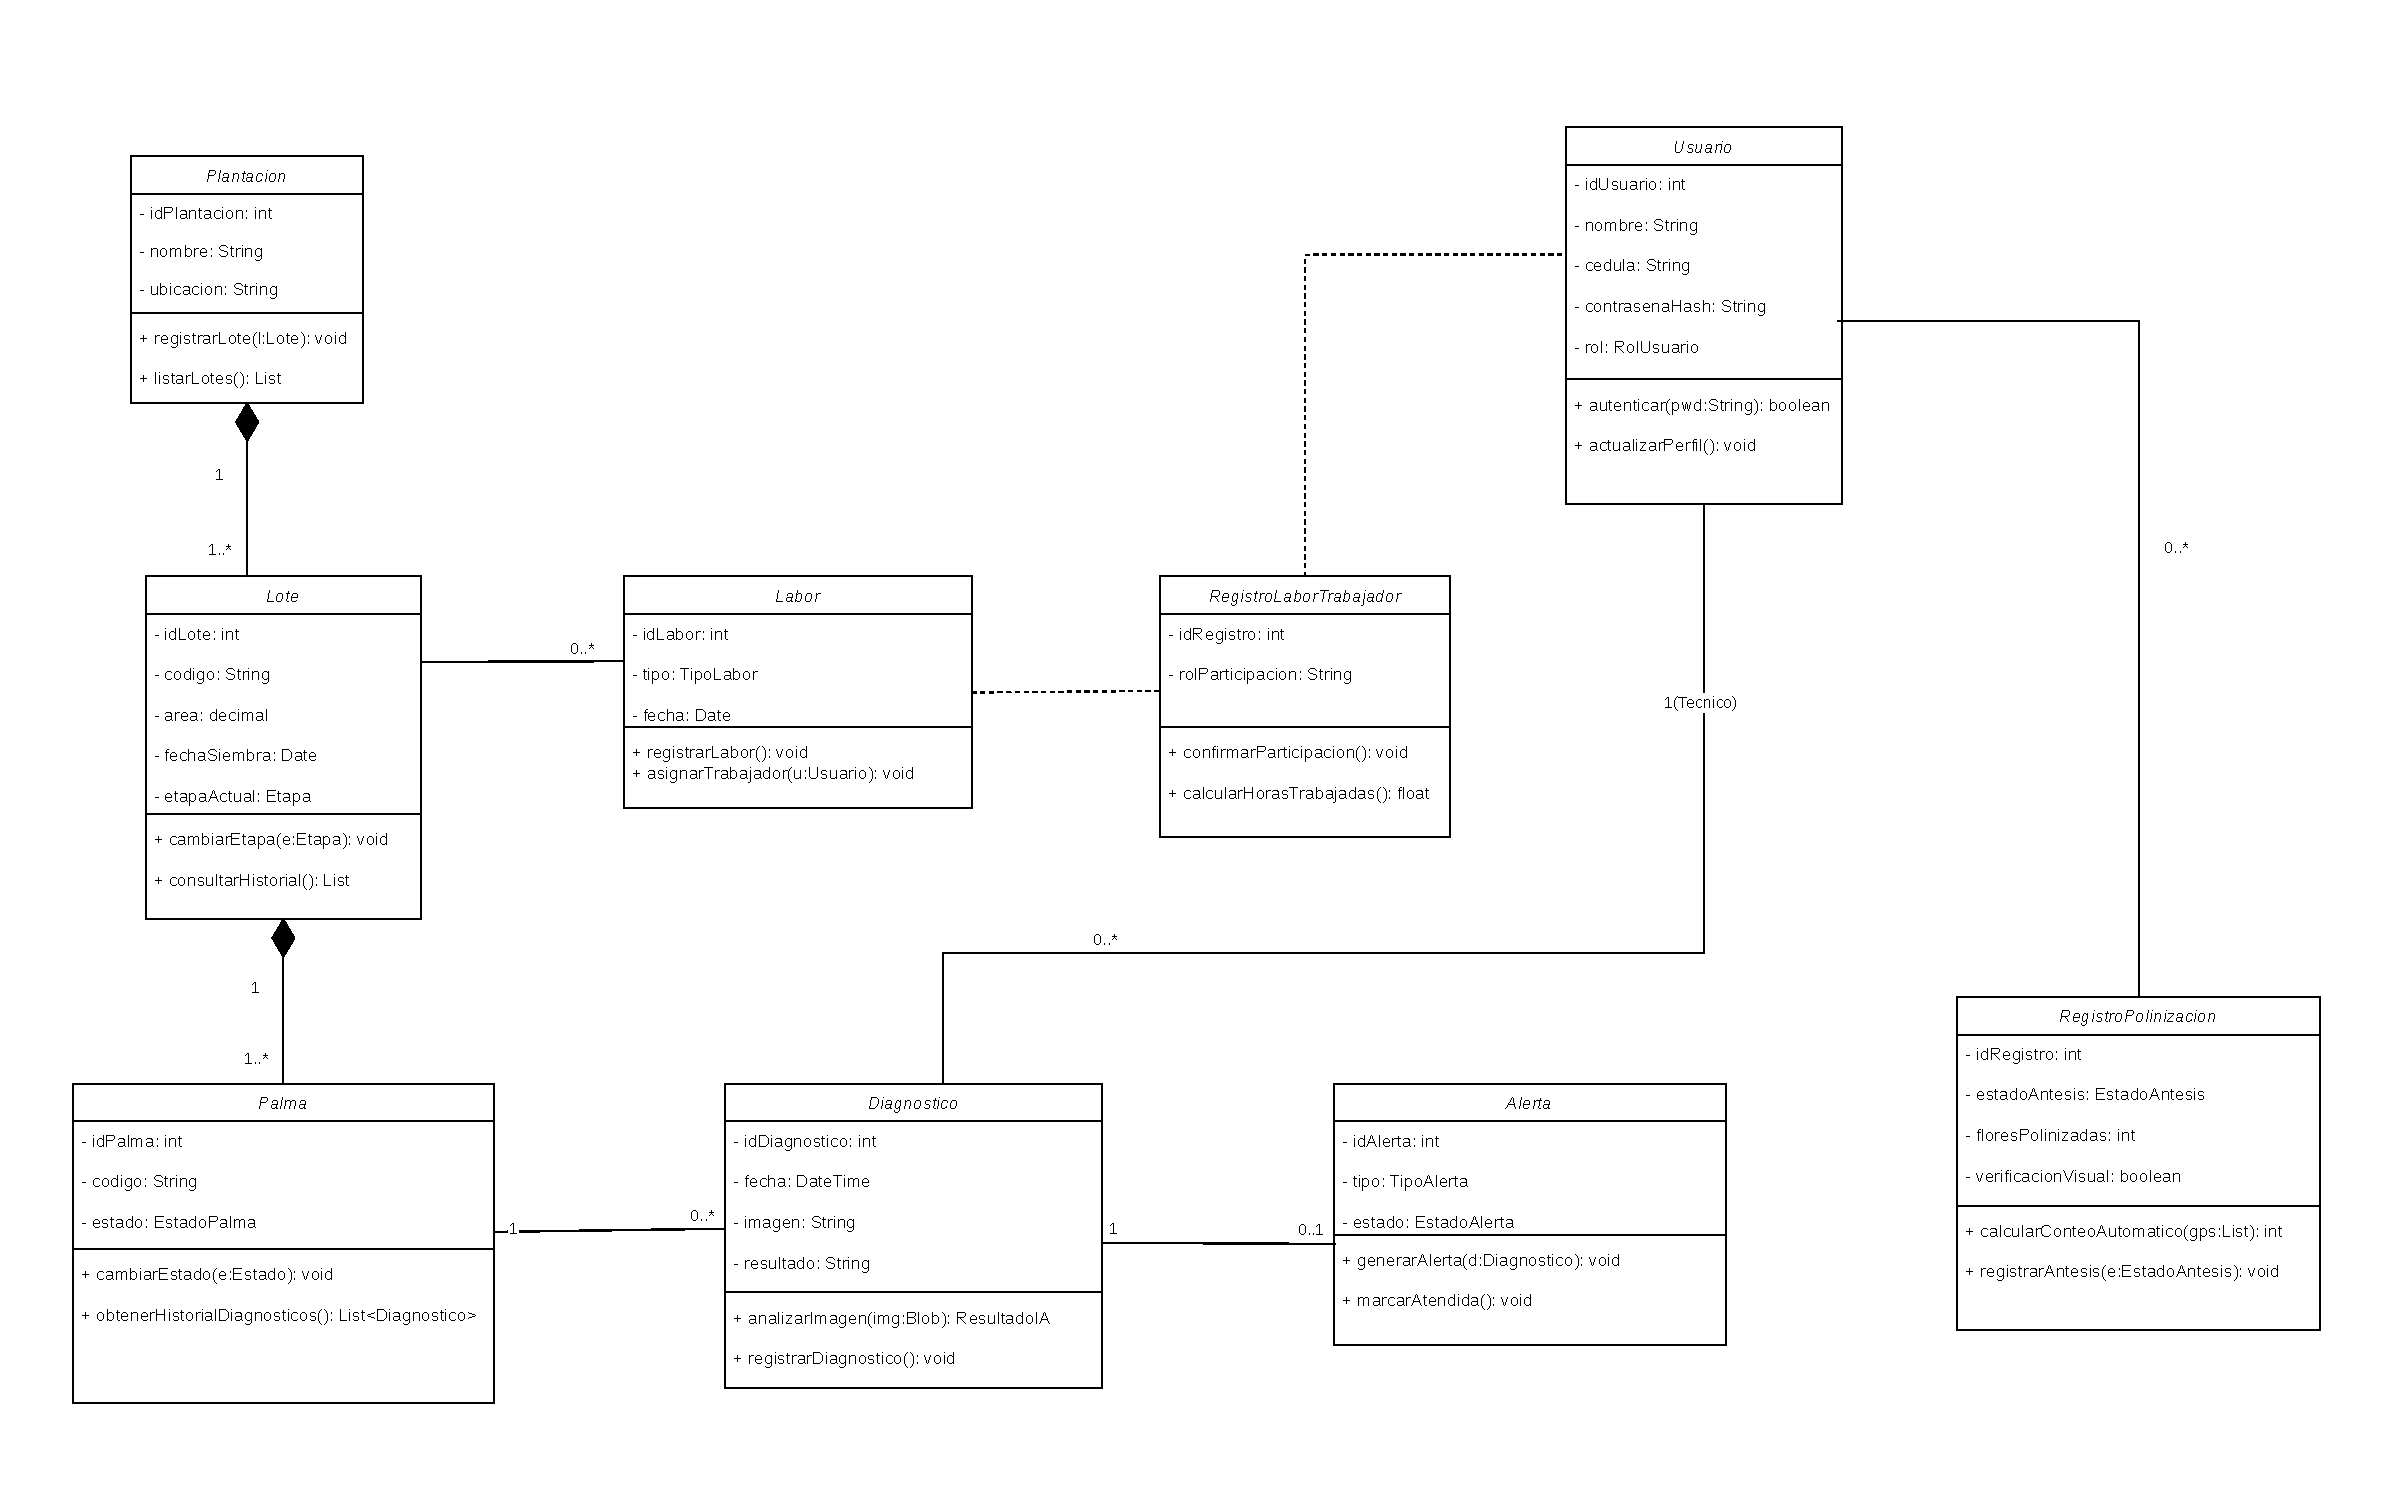
\includegraphics[width=\linewidth]{imagenes/Diagrama-Clases.drawio.pdf}
\label{fig:diagrama-estados}
\end{figure}


  
  \item Diagrama de Clases UML (\texttt{Entidad-Relacion.drawio.pdf}) -- Figura~\ref{fig:diagrama-clases}, página~\pageref{fig:diagrama-clases}.

 \begin{figure}[H]
\centering
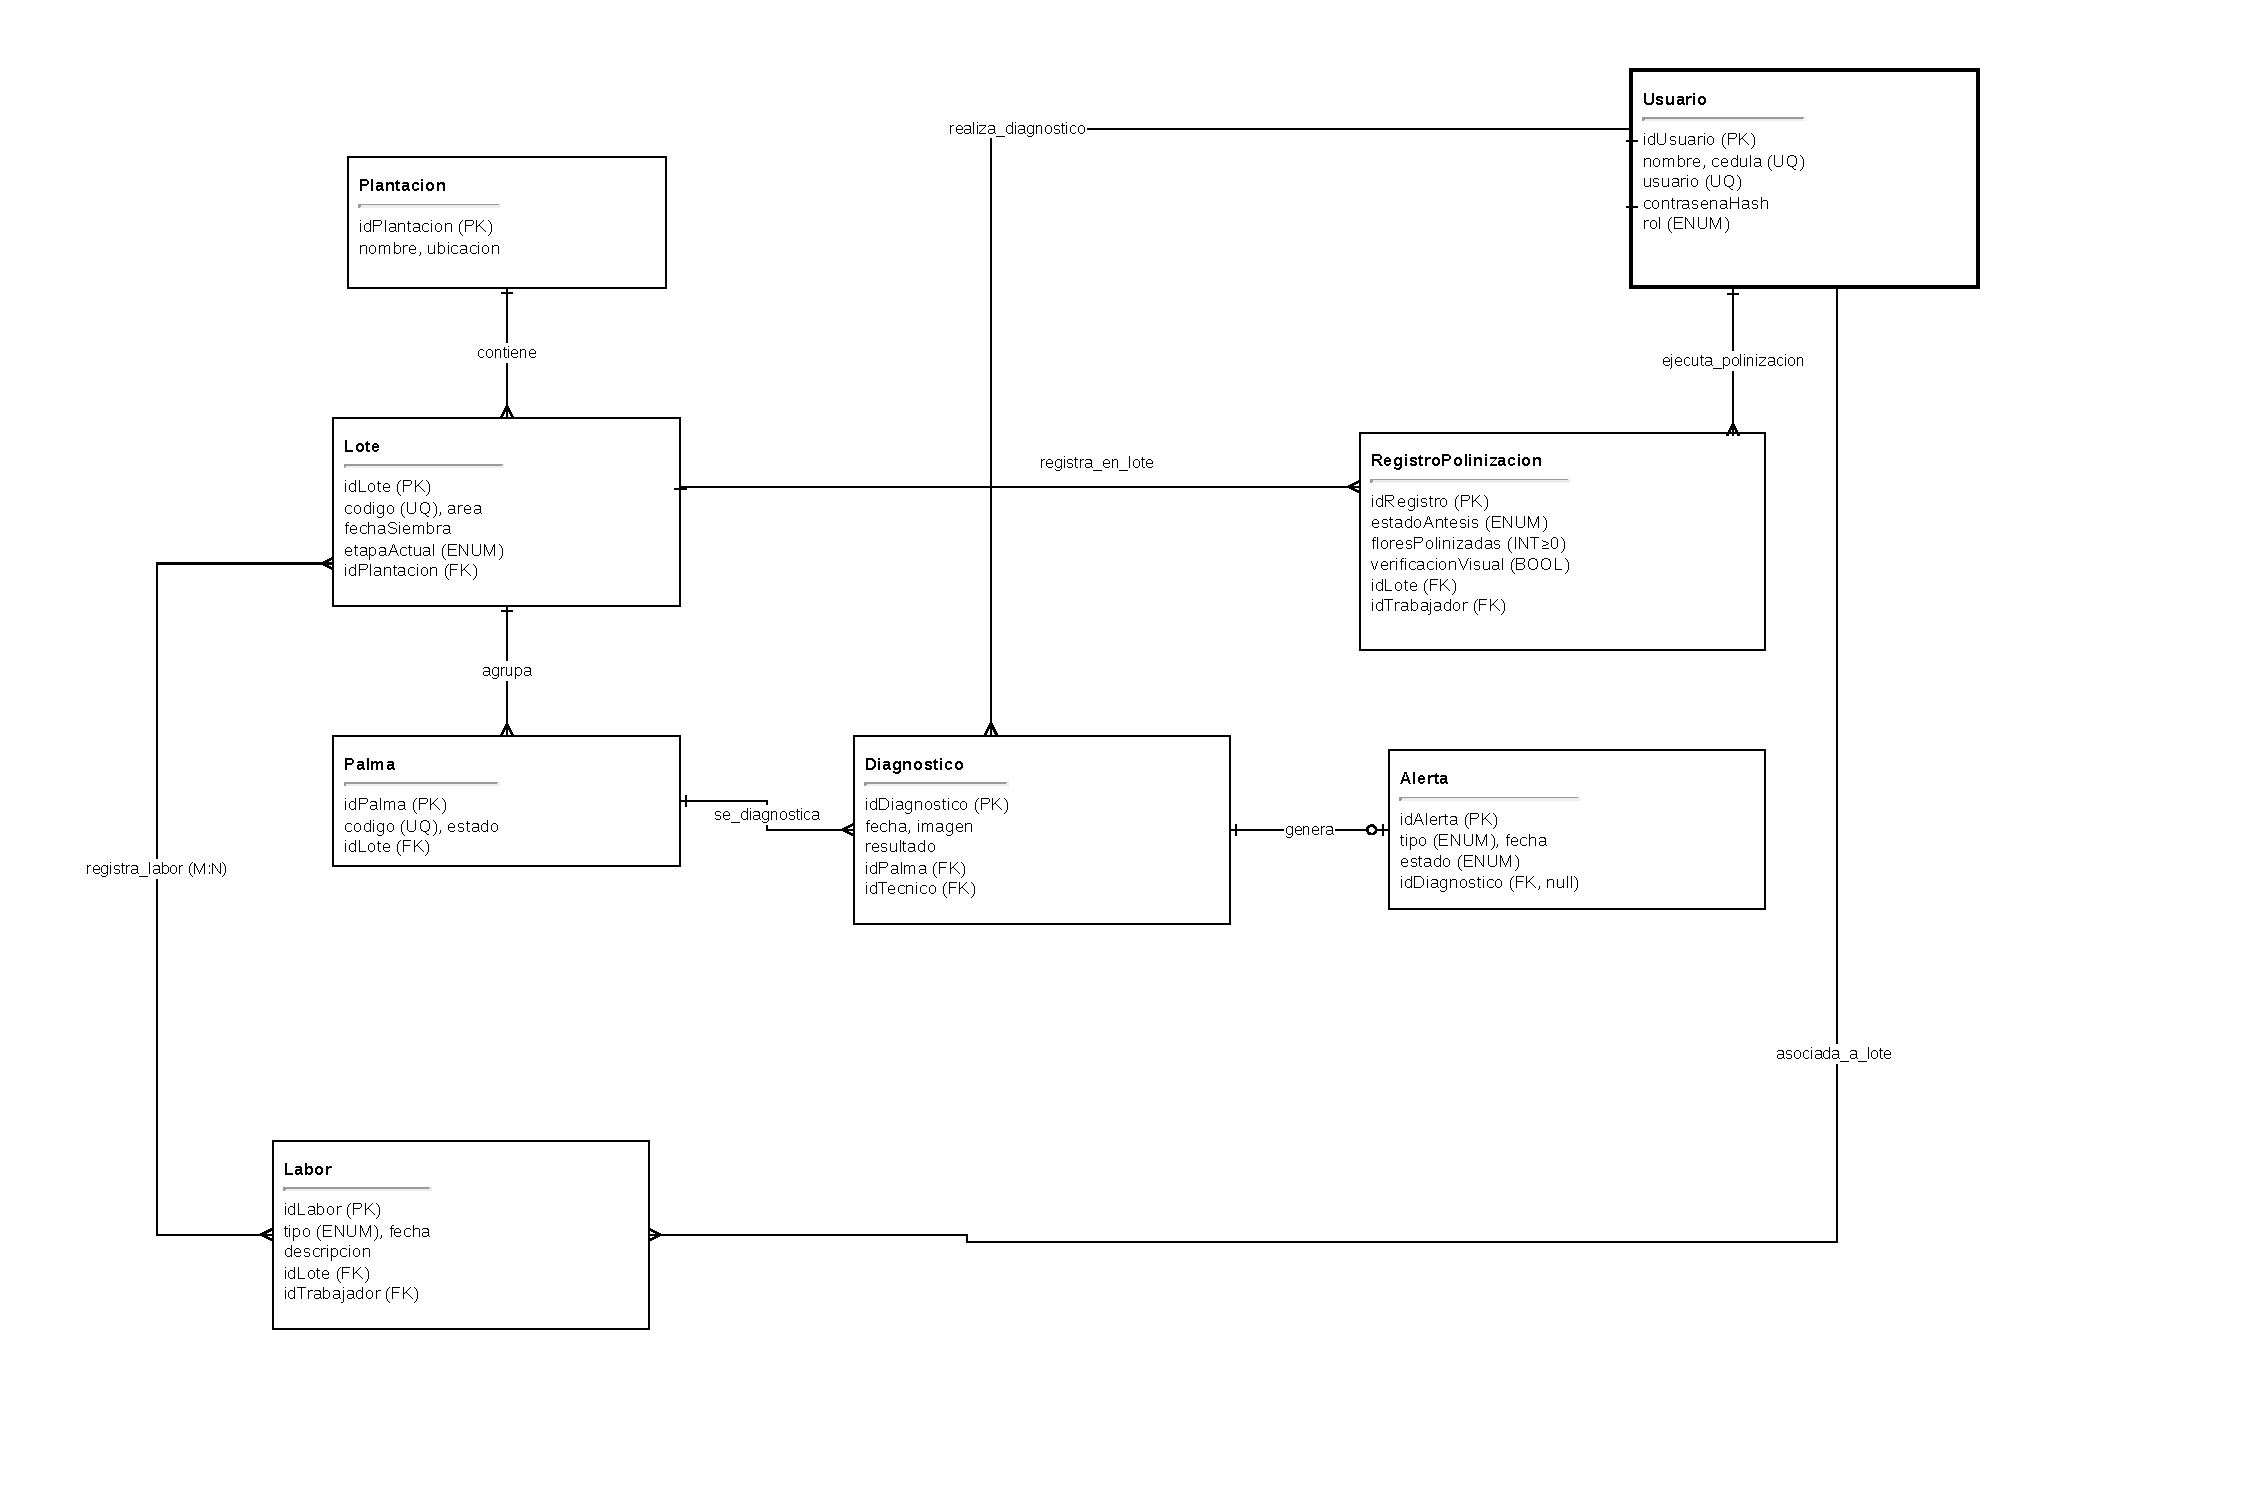
\includegraphics[width=\linewidth]{imagenes/Entidad-Relacion.drawio.pdf}

\label{fig:diagrama-estados}
\end{figure}

  \item DFD Nivel 0 (\texttt{imagenes/Diagrama-DFD0.drawio.pdf}) -- Figura~\ref{fig:dfd-nivel0}, página~\pageref{fig:dfd-nivel0}.

   \begin{figure}[H]
\centering
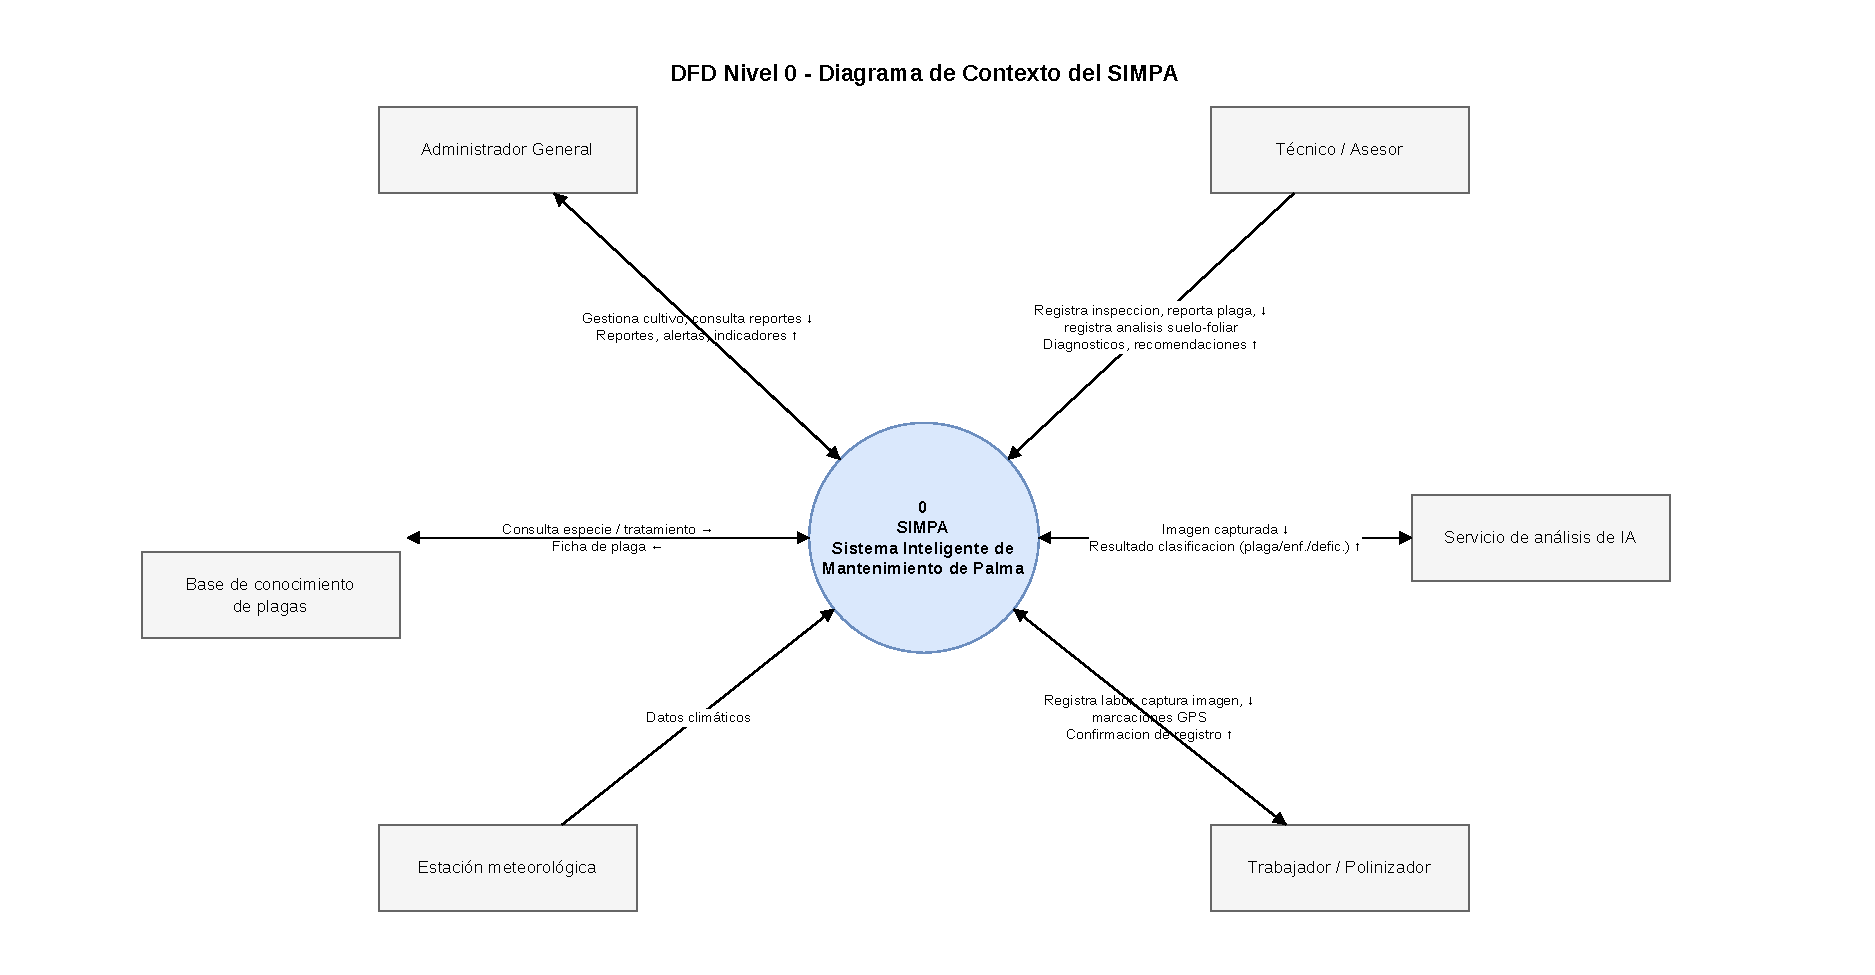
\includegraphics[width=\linewidth]{imagenes/Diagrama-DFD0.drawio.pdf}
\label{fig:diagrama-estados}
\end{figure}

  \item DFD Nivel 1 (\texttt{imagenes/Diagrama-DFD1.drawio.pdf}) -- Figura~\ref{fig:dfd-nivel1}, página~\pageref{fig:dfd-nivel1}.

   \begin{figure}[H]
\centering
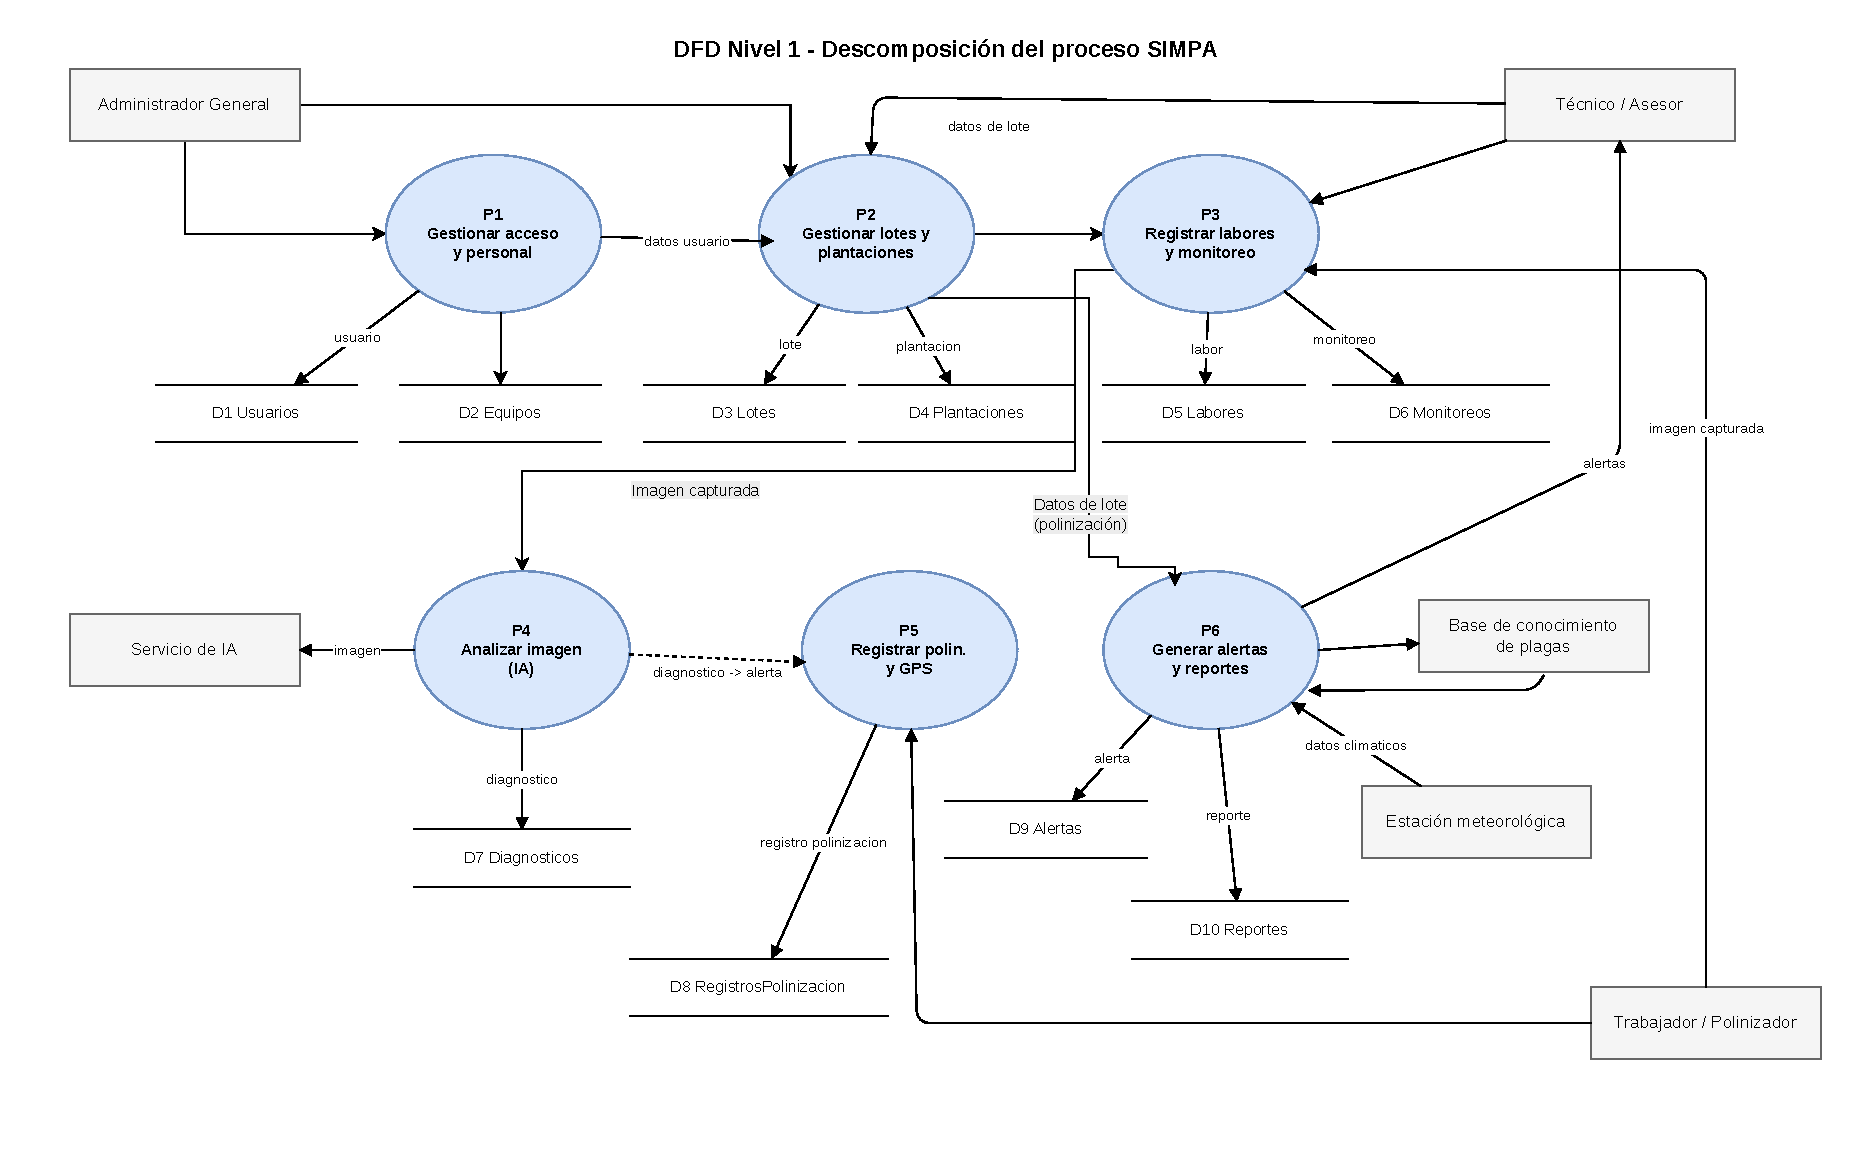
\includegraphics[width=\linewidth]{imagenes/Diagrama-DFD1.drawio.pdf}
\label{fig:diagrama-estados}
\end{figure}

  \item DFD Esencial (\texttt{imagenes/Diagrama-DFDEsencial.drawio.pdf}) -- Figura~\ref{fig:dfd-esencial}, página~\pageref{fig:dfd-esencial}.

   \begin{figure}[H]
\centering
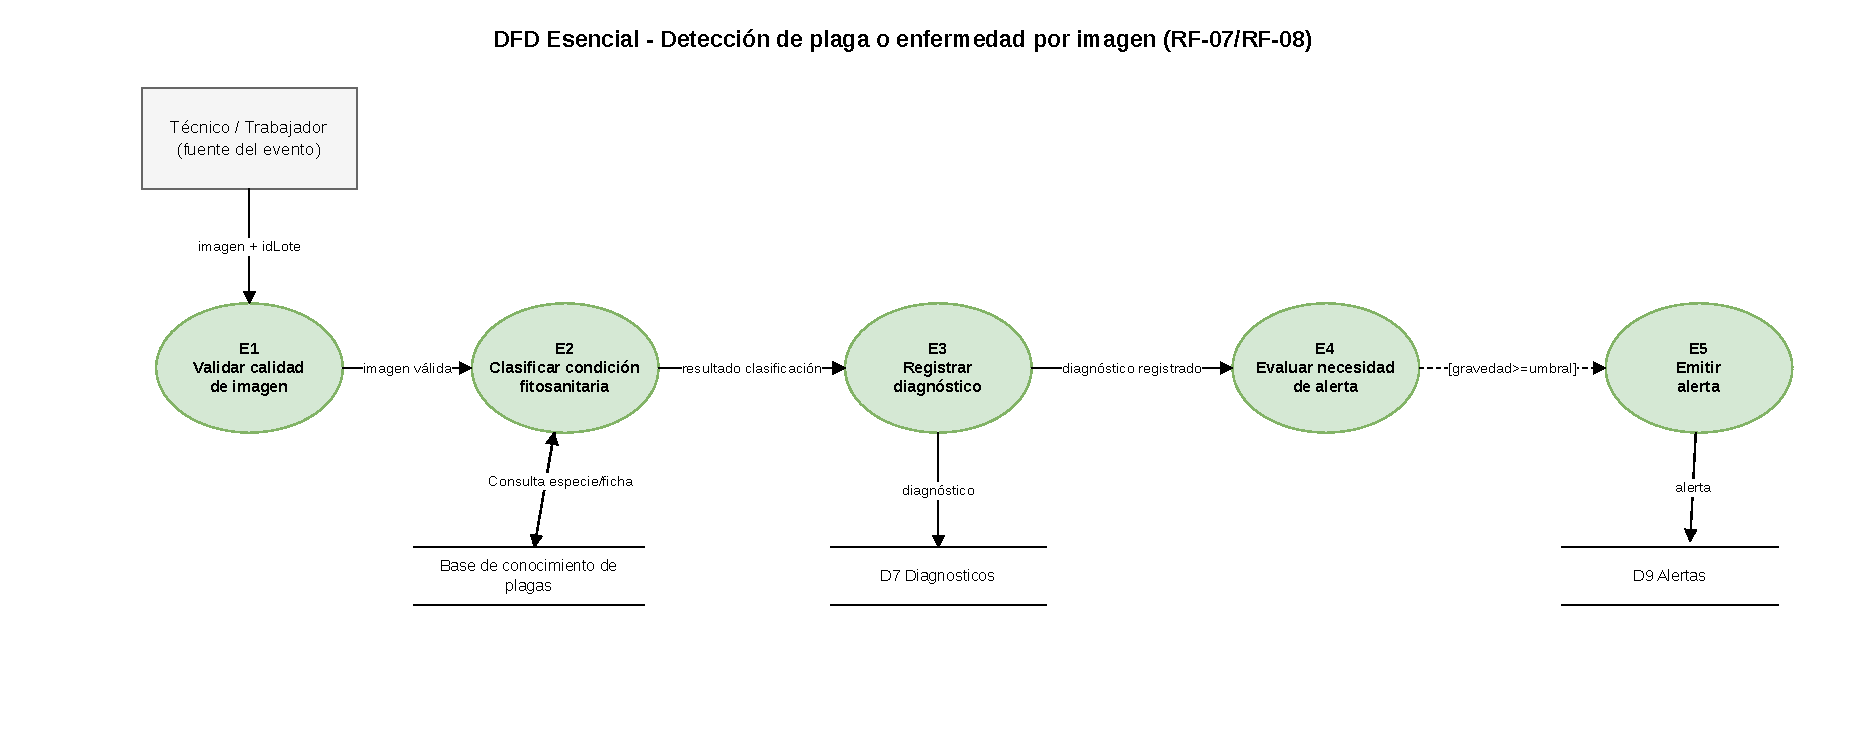
\includegraphics[width=\linewidth]{imagenes/Diagrama-DFDEsencial.drawio.pdf}
\label{fig:diagrama-estados}
\end{figure}

  \item Diagrama de Actividades (\texttt{imagenes/Diagrama-Actividades.drawio}) -- Figura~\ref{fig:diagrama-actividades}, página~\pageref{fig:diagrama-actividades}.

   \begin{figure}[H]
\centering
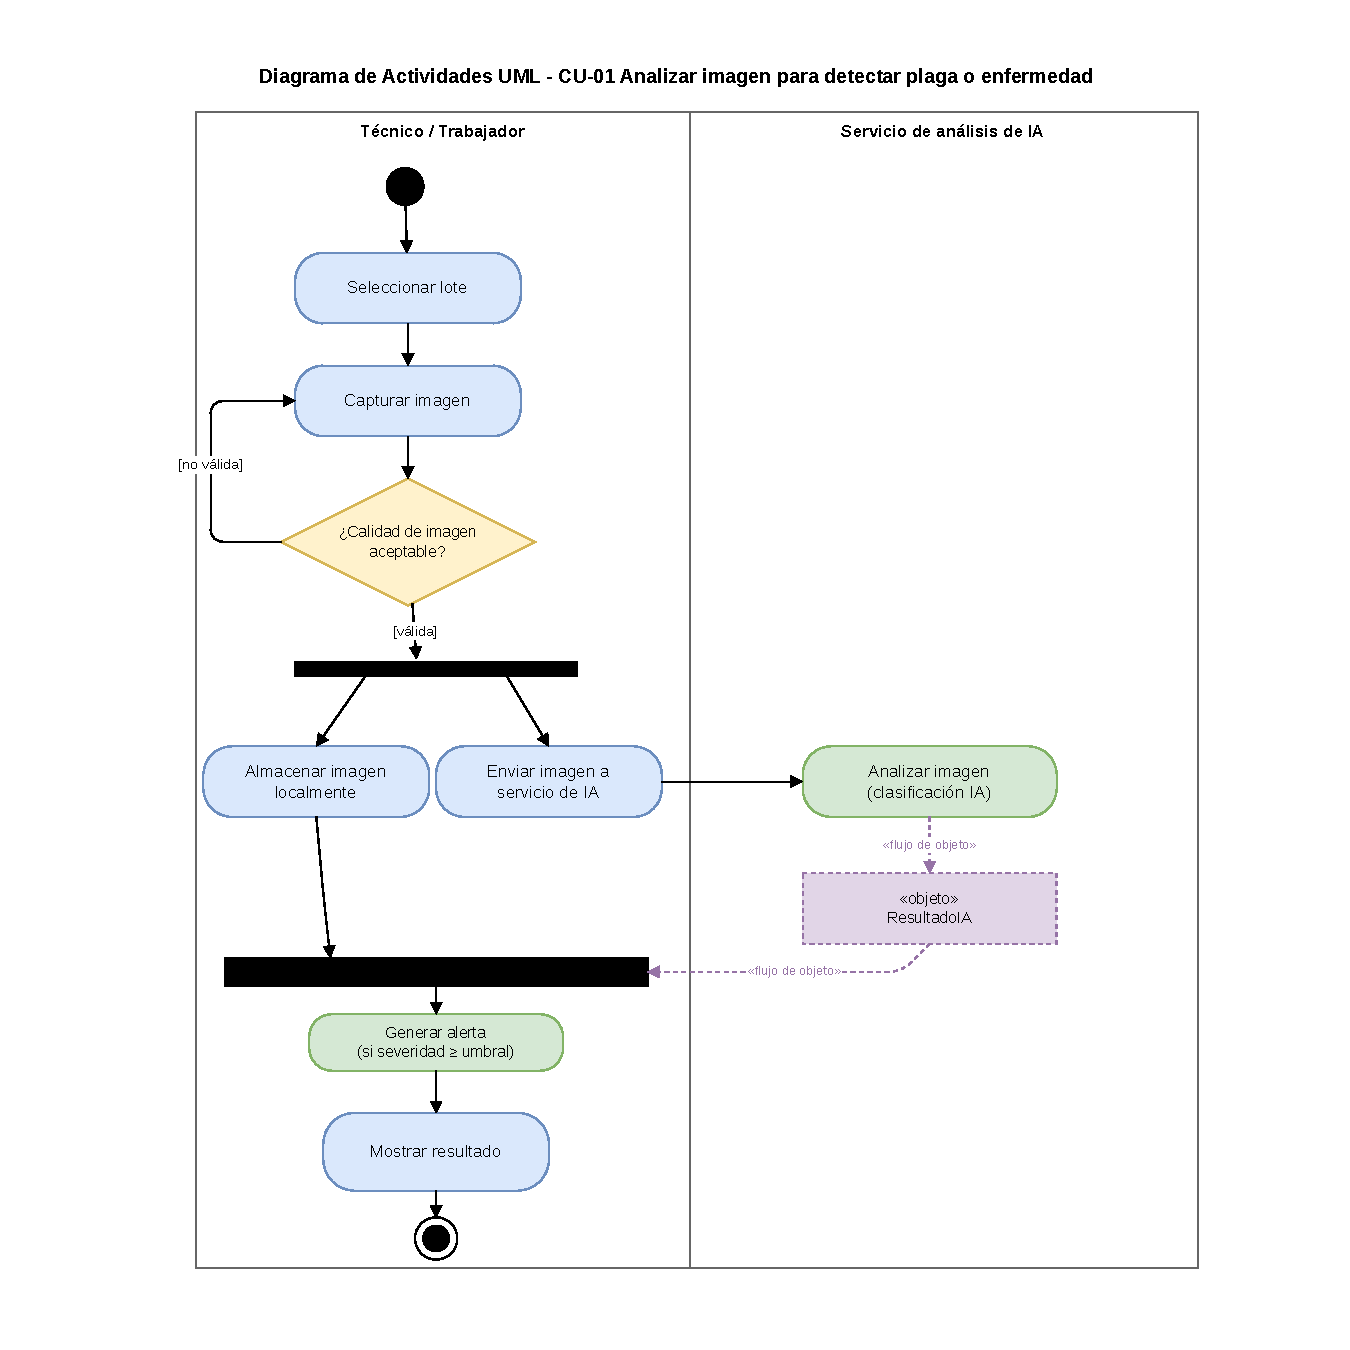
\includegraphics[width=\linewidth]{imagenes/Diagrama-Actividades.drawio}
\label{fig:diagrama-estados}
\end{figure}

  \item Diagrama de Máquina de Estados (\texttt{imagenes/Diagrama-Estados.drawiof}) -- Figura~\ref{fig:diagrama-estados}, página~\pageref{fig:diagrama-estados}.

   \begin{figure}[H]
\centering
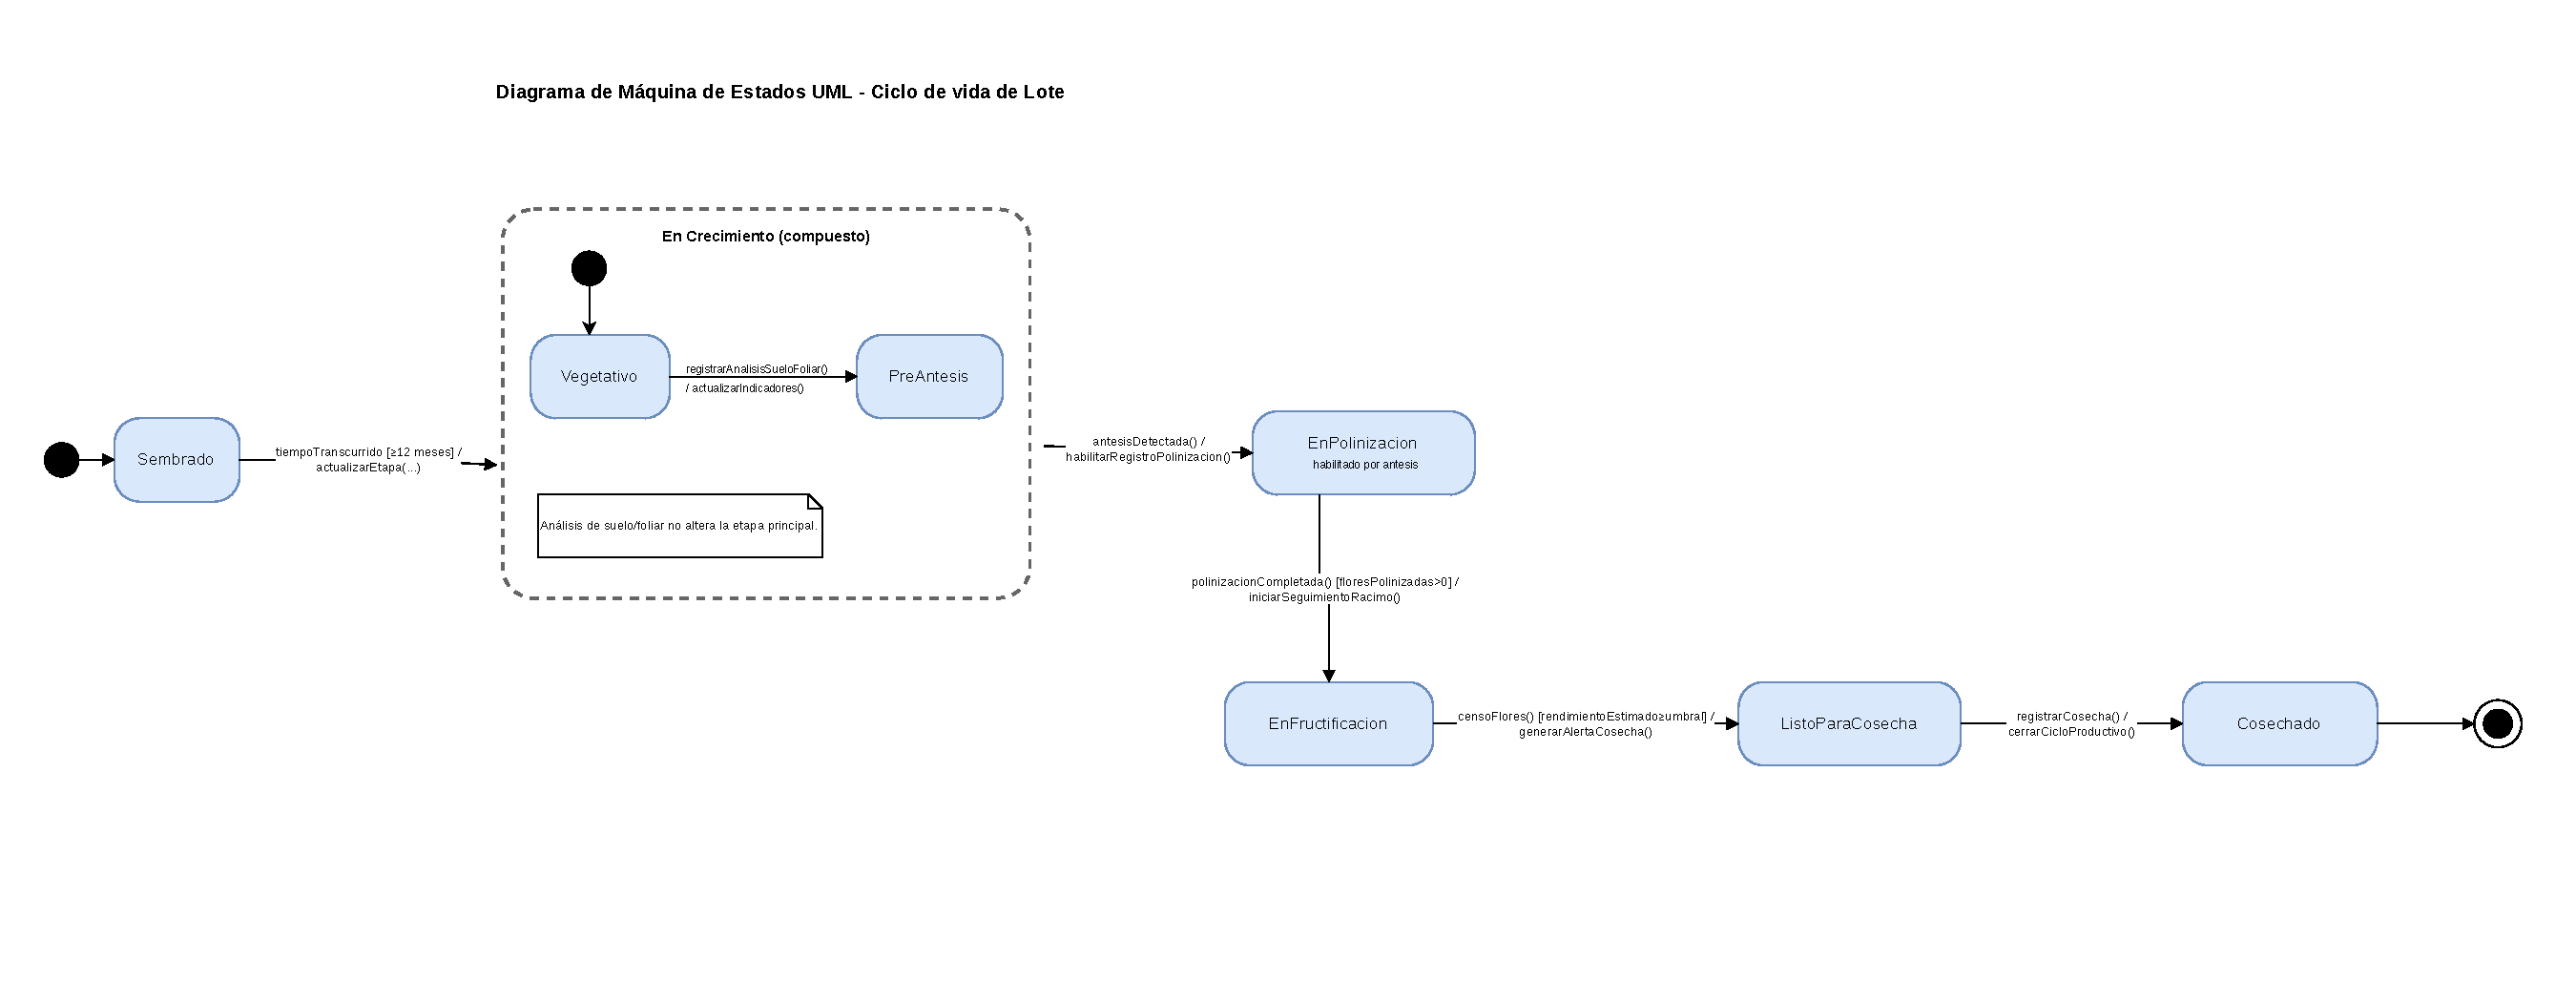
\includegraphics[width=\linewidth]{imagenes/Diagrama-Estados.drawio}
\label{fig:diagrama-estados}
\end{figure}

  \item Diagrama de Secuencia (\texttt{imagenes/Diagrama-Secuencia.drawio.pdf}) -- Figura~\ref{fig:diagrama-secuencia}, página~\pageref{fig:diagrama-secuencia}.

   \begin{figure}[H]
\centering
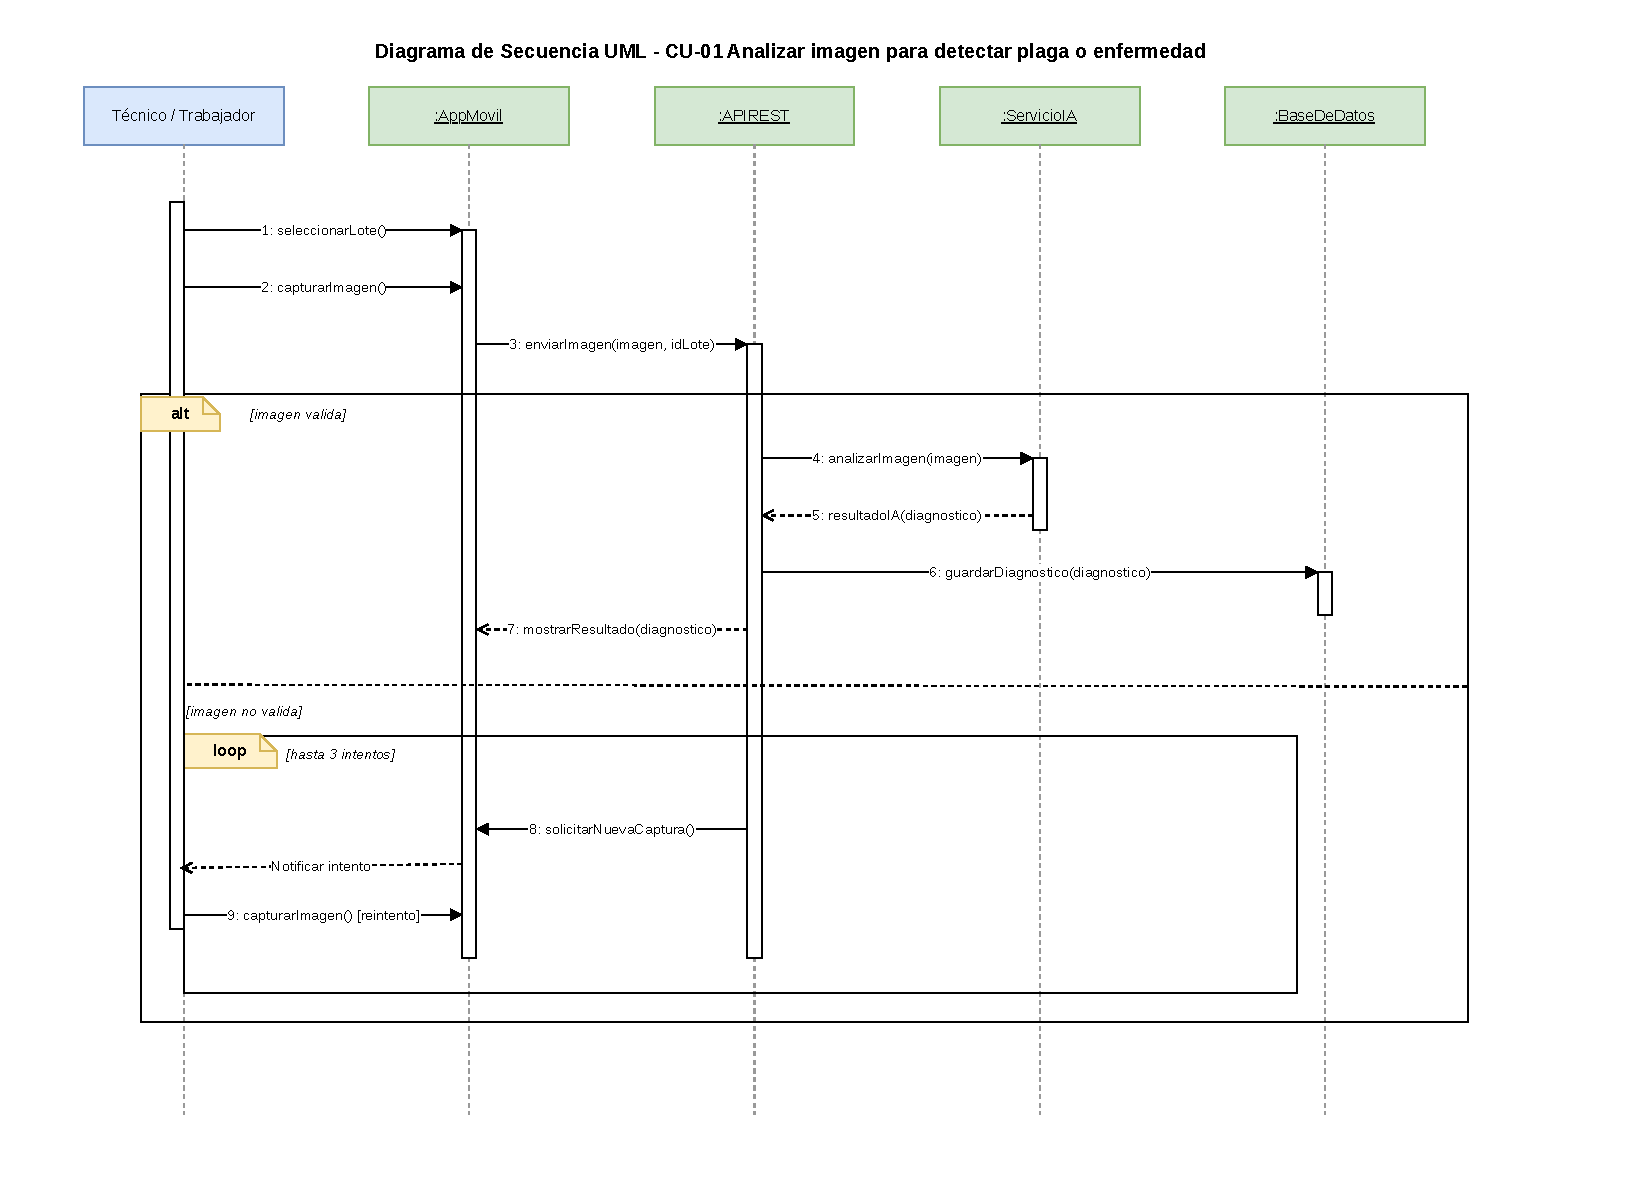
\includegraphics[width=\linewidth]{imagenes/Diagrama-Secuencia.drawio.pdf}
\label{fig:diagrama-estados}
\end{figure}

\end{itemize}
\chapter{Referencias IEEE y declaración de uso de IA}

\section{Declaración de uso de inteligencia artificial}

En la elaboración de este documento se utilizó un modelo de lenguaje de gran escala (Claude, de
Anthropic) como herramienta de apoyo para: (i) estructurar el documento conforme a
IEEE/ISO/IEC 29148:2018~\cite{ieee29148}; (ii) redactar la revisión de defectos y su corrección en
sintaxis EARS~\cite{mavin2009} a partir de los requisitos ya formalizados en la Entrega 1B del PFC;
(iii) proponer la tabla de atributos, el modelo entidad-relación, el diagrama de clases, los DFD, el
diagrama de actividades, la máquina de estados, el diagrama de secuencia y la matriz de trazabilidad,
en todos los casos derivados exclusivamente del contenido del PFC del SIMPA proporcionado como fuente;
y (iv) localizar y verificar mediante búsqueda web las referencias bibliográficas adicionales con DOI
real citadas en las conclusiones y en el marco teórico. Ningún diagrama fue generado como imagen por la
IA: todos los lugares donde debe insertarse un diagrama construido en herramienta CASE (draw.io o
StarUML) se dejaron marcados explícitamente con el texto correspondiente. La revisión crítica final del
contenido, su coherencia con el PFC y la verificación de los DOI reales quedó a cargo del equipo I.

\section{Índice de referencias en formato IEEE}

Las referencias se generan automáticamente a partir de \texttt{referencias.bib} mediante
\texttt{ieeetr}. Se listan a continuación de forma resumida para verificación rápida:
   \begin{figure}[H]
\centering
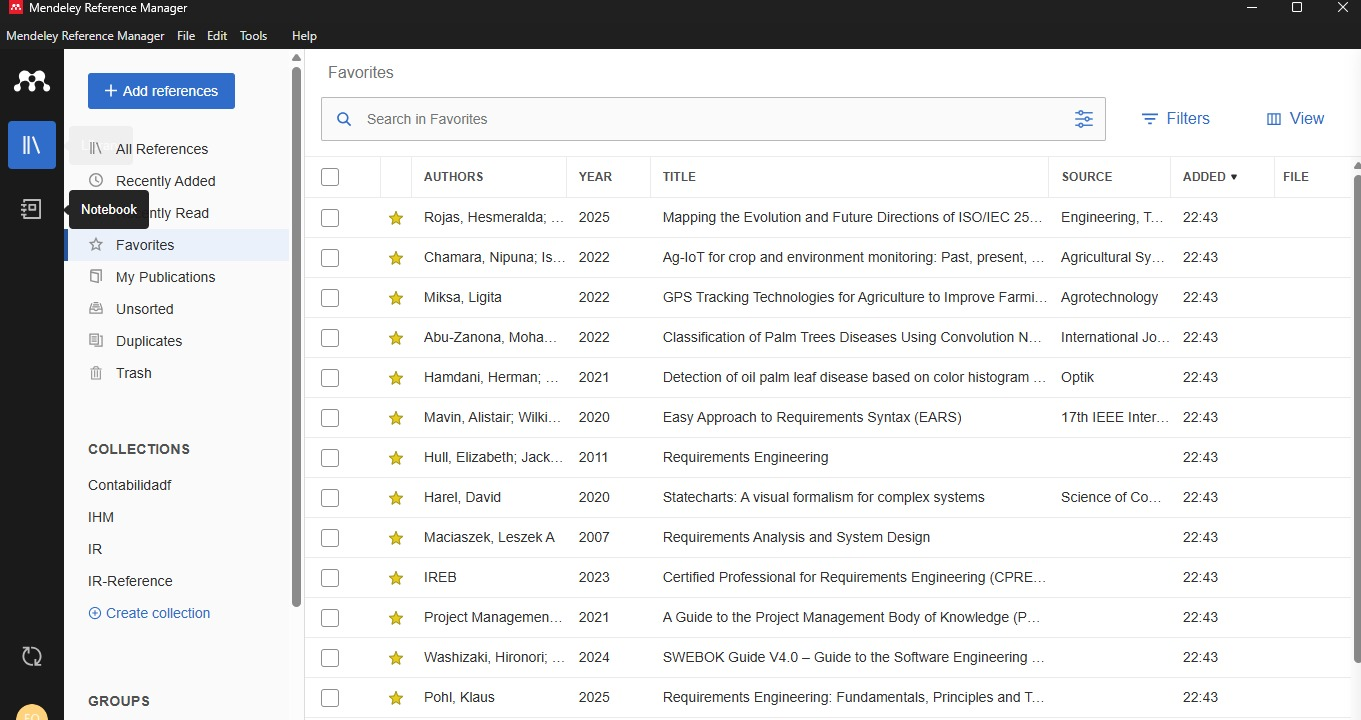
\includegraphics[width=\linewidth]{imagenes/Referencias.png}
\label{fig:diagrama-estados}
\end{figure}


\begin{enumerate}[label=\lbrack{}\arabic*\rbrack{}]
  \item IEEE/ISO/IEC 29148:2018 -- Requirements engineering.
  \item IEEE/ISO/IEC 15288:2023 -- System life cycle processes.
  \item IEEE/ISO/IEC 12207:2017 -- Software life cycle processes.
  \item ISO/IEC 25010:2023 -- SQuaRE product quality model.
  \item K. Pohl, \textit{Requirements Engineering}, 2.\textsuperscript{a} ed., Springer, 2025.
  \item SWEBOK Guide V4.0, IEEE Computer Society, 2024.
  \item PMBoK Guide, 7.\textsuperscript{a} ed., PMI, 2021.
  \item IREB CPRE Foundation Level Syllabus v3.1, 2023.
  \item L. A. Maciaszek, \textit{Requirements Analysis and System Design}, 3.\textsuperscript{a} ed.,
  Addison-Wesley, 2020.
  \item D. Harel, ``Statecharts,'' \textit{Science of Computer Programming}, 2020,
  doi: 10.1016/0167-6423(87)90035-9.
  \item E. Hull, K. Jackson, J. Dick, \textit{Requirements Engineering}, 3.\textsuperscript{a} ed.,
  Springer, 2011, doi: 10.1007/978-1-84996-405-0.
  \item A. Mavin et al., ``EARS,'' RE'09, 2009, doi: 10.1109/RE.2009.9.
  \item M. Abu-Zanona et al., ``Classification of Palm Trees Diseases Using CNN,'' IJACSA, 2022,
  doi: 10.14569/ijacsa.2022.01306111.
  \item H. Hamdani et al., ``Detection of oil palm leaf disease,'' Optik, 2021,
  doi: 10.1016/j.ijleo.2021.167753.
  \item L. Miksa, ``GPS Tracking Technologies for Agriculture,'' Agrotechnology, 2022,
  doi: 10.35248/2168-9881.22.11.286.
  \item N. Chamara et al., ``Ag-IoT for crop and environment monitoring,'' Agricultural Systems, 2022,
  doi: 10.1016/j.agsy.2022.103497.
  \item H. Rojas et al., ``Mapping the Evolution of ISO/IEC 25010,'' ETASR, 2025,
  doi: 10.48084/etasr.11772.
\end{enumerate}

\end{document}
